\chapter{Appendix: Real-Time Demonstration of Optical Communication System Using HpCom Simulator}

This interactive demonstration offers a unique, real-time exploration of optical communication system simulations, powered by the High-Performance COMmunication (HpCom) library (Fig.~\ref{fig:HpCom_scheme}). Participants can witness first-hand the effects of system parameters and signal processing techniques on image quality, transforming a photograph taken at our stand into a vivid illustration of optical communication complexities.

In the rapidly advancing domain of optical communication systems, efficient, high-performance simulation tools are of critical importance. Recognizing the need for a software tailored to the demands of this field, we introduce our GPU-accelerated HpCom library\cite{esf0_2023_7880552}. This framework enhances simulation capabilities, fostering innovation and accelerating research.

The use of GPUs in our library provides significant advantages, such as parallel computations, scalability, and power efficiency. These aspects enable efficient handling of large-scale computations, an essential feature for researchers tackling the computational demands of emerging optical communication systems.

Our demo serves as an educational platform, illustrating how GPU-based simulations allow researchers to explore varied scenarios quickly and efficiently, leading to faster discoveries and more effective resource utilization. As participants interact with the demo, they will gain a tangible understanding of the impacts of system parameter changes and advanced techniques on signal quality.



\section{Procedure}

The primary objective of this demonstration is to showcase the speed of our numerical simulations. To emphasize this, we propose a demonstration procedure in which each stage takes no more than a few dozen seconds, contingent on the specific system parameters.

% The process begins by taking a picture of the participant, which is then uploaded to a server. This image will be decomposed into bits, including all RGB components, and utilized as the payload for numerical simulations. The web interface allows for modification of various simulation parameters such as the number of spans, dispersion, average power, and noise.

\textbf{1. Image Capture and Conversion:} A visitor to the stand has their photograph taken. This digital image, composed of a matrix of pixels, is then transformed into binary data. Every pixel, composed of red, green, and blue (RGB) colour components, is broken down into its RGB values. These values are then converted into binary format, generating a long bit stream that serves as the payload for the ensuing simulation.


\begin{figure}[t]
   \centering
        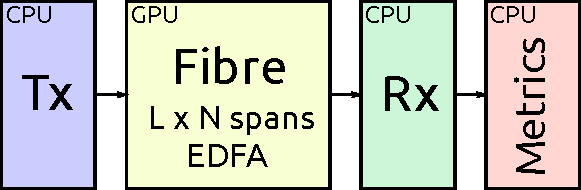
\includegraphics[width=0.7\linewidth]{images/hpcom/hpcom_scheme.pdf}
    \caption{Framework architecture for optical communication system simulation, featuring optimized transceiver (Tx) design, GPU-accelerated SSFM-based channel model (with $N$ spans of length $L$), receiver implementation (Rx), and performance metrics evaluation including BER, EVM, and MI.}
    \label{fig:HpCom_scheme}
\end{figure}

\textbf{2. Setting Simulation Parameters:} The visitor is invited to interact with our intuitive web interface, designed to provide control over various simulation parameters. These parameters include:
\begin{description}[style=multiline, leftmargin=4cm, font=\normalfont]
    \item[\texttt{Average power}] The mean optical power launched into the fibre in dBm. Default $P_{ave}=0$ \textrm{[dBm]}.
    \item[\texttt{Modulation format}] The optical modulation scheme used to encode the data. Possible values are 4-, 16-, 64-, 256- and 1024-QAM.
    \item[\texttt{Symbol frequency}] Symbol frequency in GHz. Default is 34 \textrm{[GHz]}.
    \item[\texttt{Number of spans}] The number of optical fibre spans. Default is 12.
    \item[\texttt{Length of spans}] The length of each fibre span. Default is 80 \textrm{[km]}.
    \item[\texttt{Attenuation}] The fibre's attenuation parameter. For \gls{smf} $\alpha = 0.2$ $[\textrm{dB}/\textrm{km}]$
    \item[\texttt{Nonlinearity}] The fibre's nonlinearity parameter. For \gls{smf} $\gamma = 1.2$ $[\textrm{W} \cdot \textrm{km}]^{-1}$.
    \item[\texttt{Noise}] The amplified spontaneous emission (ASE) noise from the erbium-doped fibre amplifiers (EDFAs). Default value is 4.5 \textrm{[dB]}. For system without noise big negative value is used, e.g. -200.
    \item[\texttt{Dispersion}] The fibre's chromatic dispersion parameter. For \gls{smf} $D = 16.8$ $\textrm{ps}/[\textrm{nm} \cdot \textrm{km}]$.
    \item[\texttt{Simulation step}] Length of simulation step in km. Default is 5 \textrm{[km]}.
\end{description}


\textbf{3. Signal Generation and Propagation:} Once the parameters are set, the HpCom library generates the signal according to the selected modulation format and propagates it through the simulated optical fibre. The library employs the Split-Step Fourier method to accurately simulate the combined effects of chromatic dispersion, nonlinearity, and noise. 



\textbf{4. Decoding and Visualization:} After the signal propagation, the signal is received on the receiver, where a corresponding matched filter is applied, followed by equalisation and demodulation. The resulting bit stream is transformed back into the RGB image data, which is rendered on the screen. The image is likely to show distortions due to the impairments introduced during signal propagation, as no Forward Error Correction (FEC) is applied.

\textbf{5. Application of Advanced Techniques:} To demonstrate how advanced signal processing techniques can improve the system performance, visitors are given the option to enable these strategies. This includes Machine Learning techniques for impairment mitigation and Digital Back Propagation (DBP) to compensate for the combined effects of chromatic dispersion and nonlinearity. The number of DBP steps per span can also be adjusted for optimal performance.


Throughout the demo, the impact of various parameters and techniques on the resulting image quality is clearly observable, providing visitors with a tangible understanding of optical communication systems' complexity. By comparing the initial and final images, they can directly see the effects of their chosen settings. The demo's real-time and interactive nature makes it a unique educational tool for those interested in optical communications.


% \section{Simulation and Decoding}

% The signal then undergoes propagation, with the option to decode without Forward Error Correction (FEC), using only Chromatic Dispersion Compensation (CDC). This simulation allows the observation of how the image quality deteriorates due to non-linear effects and other system impairments.

% \section{Analysis}

% Subsequently, the image is restored, and the impact of the chosen parameters is evident. The initial image and the simulated output can be compared directly. By introducing ML techniques, DBP, and other advanced strategies, participants can observe how these improvements enhance the quality of the transmitted image.

\section{Interface}

The practical setup is structured as follows: The React frontend manages the web interface, parameter input, log display, and selection of images. The backend comprises a Telegram bot that receives and stores images sent from a mobile camera, a Flask backend to manage frontend changes and activate the optical channel simulation, and a simulation channel that utilizes the HpCom package for its simulations. 

Figure~\ref{fig:demo1} displays an instance of the interface with specific images and settings. The interface is primarily divided into two main sections: a \textbf{visualization section} on the left and an \textbf{information and control section} on the right.

Within the interface, the Visualization Section prominently features the "Original Image" at the top-left. This image, captured with a mobile camera, represents the initial input prior to any optical channel simulations. As example, Fig.~\ref{fig:demo1} captures a scene from the ECOC 2023 GLASGOW conference, featuring two attendees. To maintain their privacy, their faces have been tastefully blurred. Adjacent to and below this original capture are three other images, each denoting a distinct processing technique, notably "prop," "cdc," and "dbp10." The "prop" image consistently displays the aftermath of channel simulation without any equalization applied. Meanwhile, the other images have undergone various equalization procedures. Specifically, "cdc" reveals the outcome post-chromatic dispersion compensation and nonlinear phase equalization. The labels "dbp2", "dbp3", and "dbp10" depict the results of \gls{dbp} with 2, 3, and 10 steps per fiber span, respectively. The "nn" label showcases additional nonlinear distortion equalization, employing different neural networks. The precise neural network deployed aligns with the specific fiber parameters. The labels "view1" through "view4" offer alternate perspectives of the constellation post-\gls{cdc} and \gls{npe}.

Transitioning to the Information and Control Section, it encompasses details about both the utilized library and the aforementioned conference. Furthermore, it comprises a simulation parameters segment, a methods dropdown menu allowing users to select the visual representation, and a log console to track operations.


\section{Example Demonstration}

\begin{figure}[ht]
  \centering
  \begin{minipage}[c]{0.33\linewidth}
    \centering
    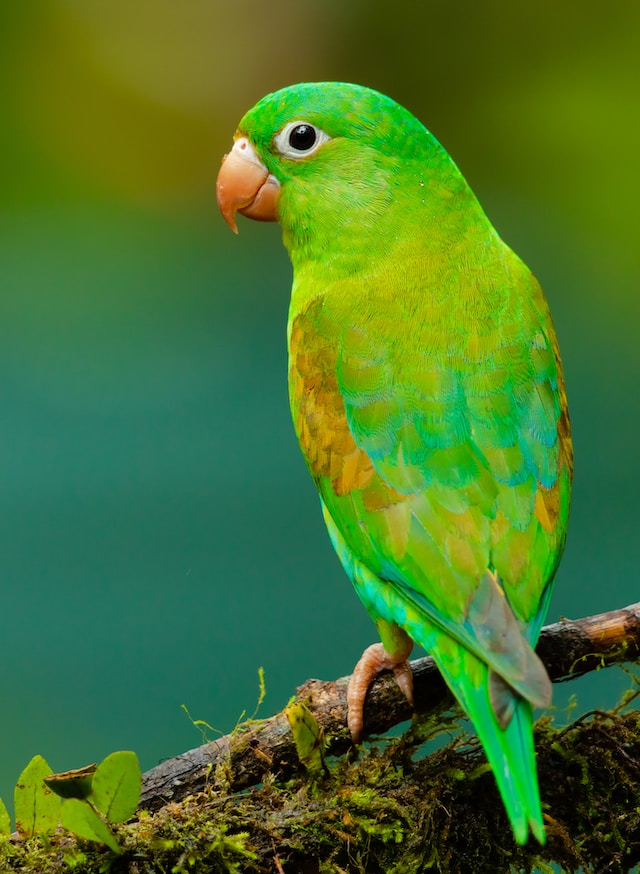
\includegraphics[width=1.\linewidth]{images/hpcom/parrot3.jpg}
  \end{minipage}
  \begin{minipage}[c]{0.33\linewidth}
    \centering
    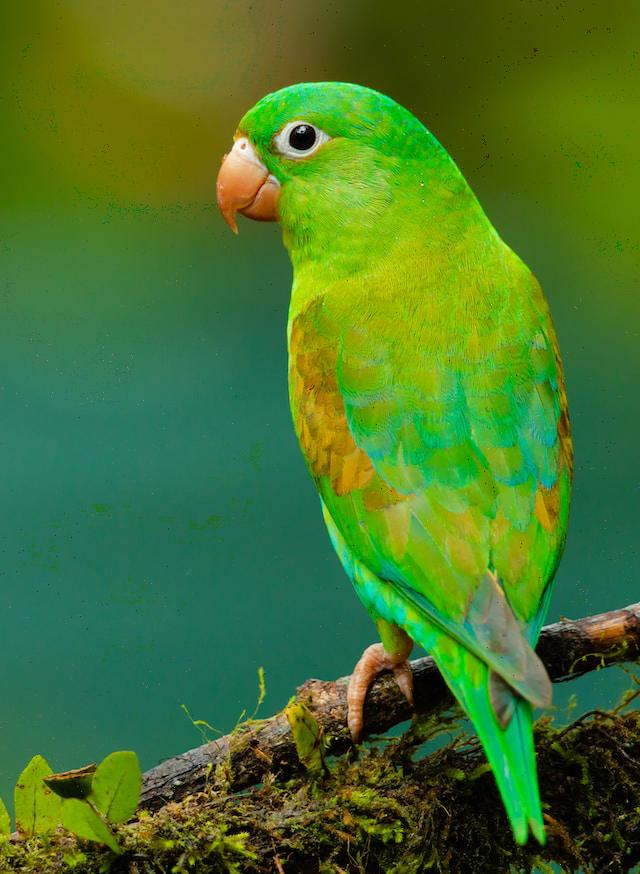
\includegraphics[width=1.\linewidth]{images/hpcom/parrot3_rx.jpg}
  \end{minipage}
  \begin{minipage}[c]{0.33\linewidth}
    \centering
    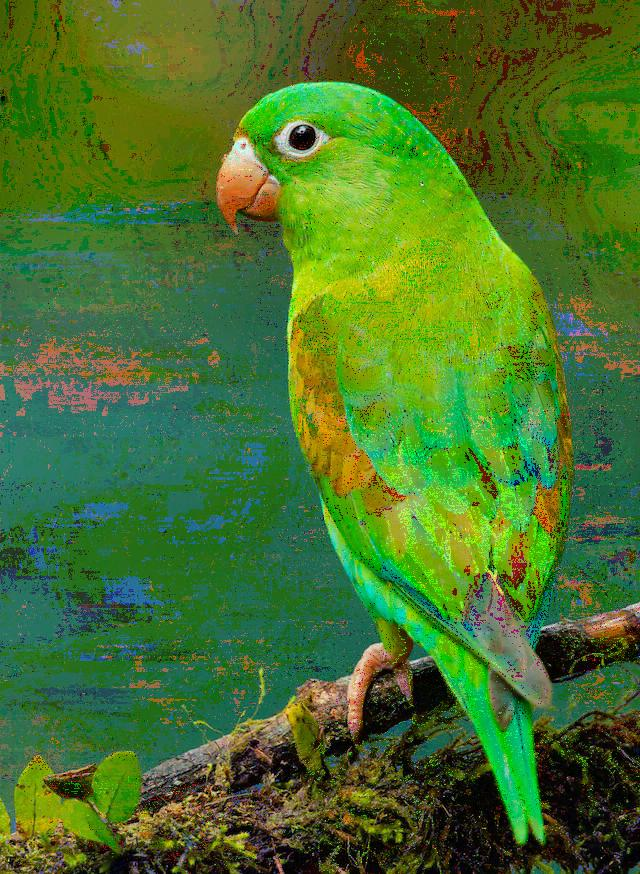
\includegraphics[width=1.\linewidth]{images/hpcom/parrot3_rx2.jpg}
  \end{minipage}
  \caption{
  The left image is the original picture to be transmitted. The central image showcases how the picture appears after signal propagation through an optical system with parameters: $P_{ave}=0$ \textrm{[dBm]}, $12 \times 80$ $[\textrm{km}]$ spans of SSFM. The fiber was characterized by an attenuation coefficient of $\alpha = 0$ $[\textrm{dB}/\textrm{km}]$, EDFA noise figure 4.5 \textrm{[dB]}, a dispersion coefficient of $D = 16.8$ $\textrm{ps}/[\textrm{nm} \cdot \textrm{km}]$, and a nonlinear coefficient of $\gamma = 1.2$ $[\textrm{W} \cdot \textrm{km}]^{-1}$. The image on the right demonstrates the when $P_{ave} = 5$ \textrm{[dBm]}.
  }
  \label{fig:demo_example}
\end{figure}

As illustrated in Fig.~\ref{fig:demo_example}, we demonstrate the process of image corruption due to signal propagation with specific system parameters. The original image of a parrot (left) undergoes signal propagation with parameters: $12 \times 80$ $[\textrm{km}]$ spans of standard single-mode fiber (SSFM), attenuation coefficient of $\alpha = 0$ $[\textrm{dB}/\textrm{km}]$, EDFA noise figure 4.5 \textrm{[dB]}, a dispersion coefficient of $D = 16.8$ $\textrm{ps}/[\textrm{nm} \cdot \textrm{km}]$, and a nonlinear coefficient of $\gamma = 1.2$ $[\textrm{W} \cdot \textrm{km}]^{-1}$. The resultant image (centre) exhibits the distortions introduced by these system parameters. Increasing the $P_{ave}$ to $5$ \textrm{[dBm]} (right image) further alters the image quality, showing how different power levels can impact the quality of the received signal.

\begin{landscape}
\begin{figure}
    \centering
    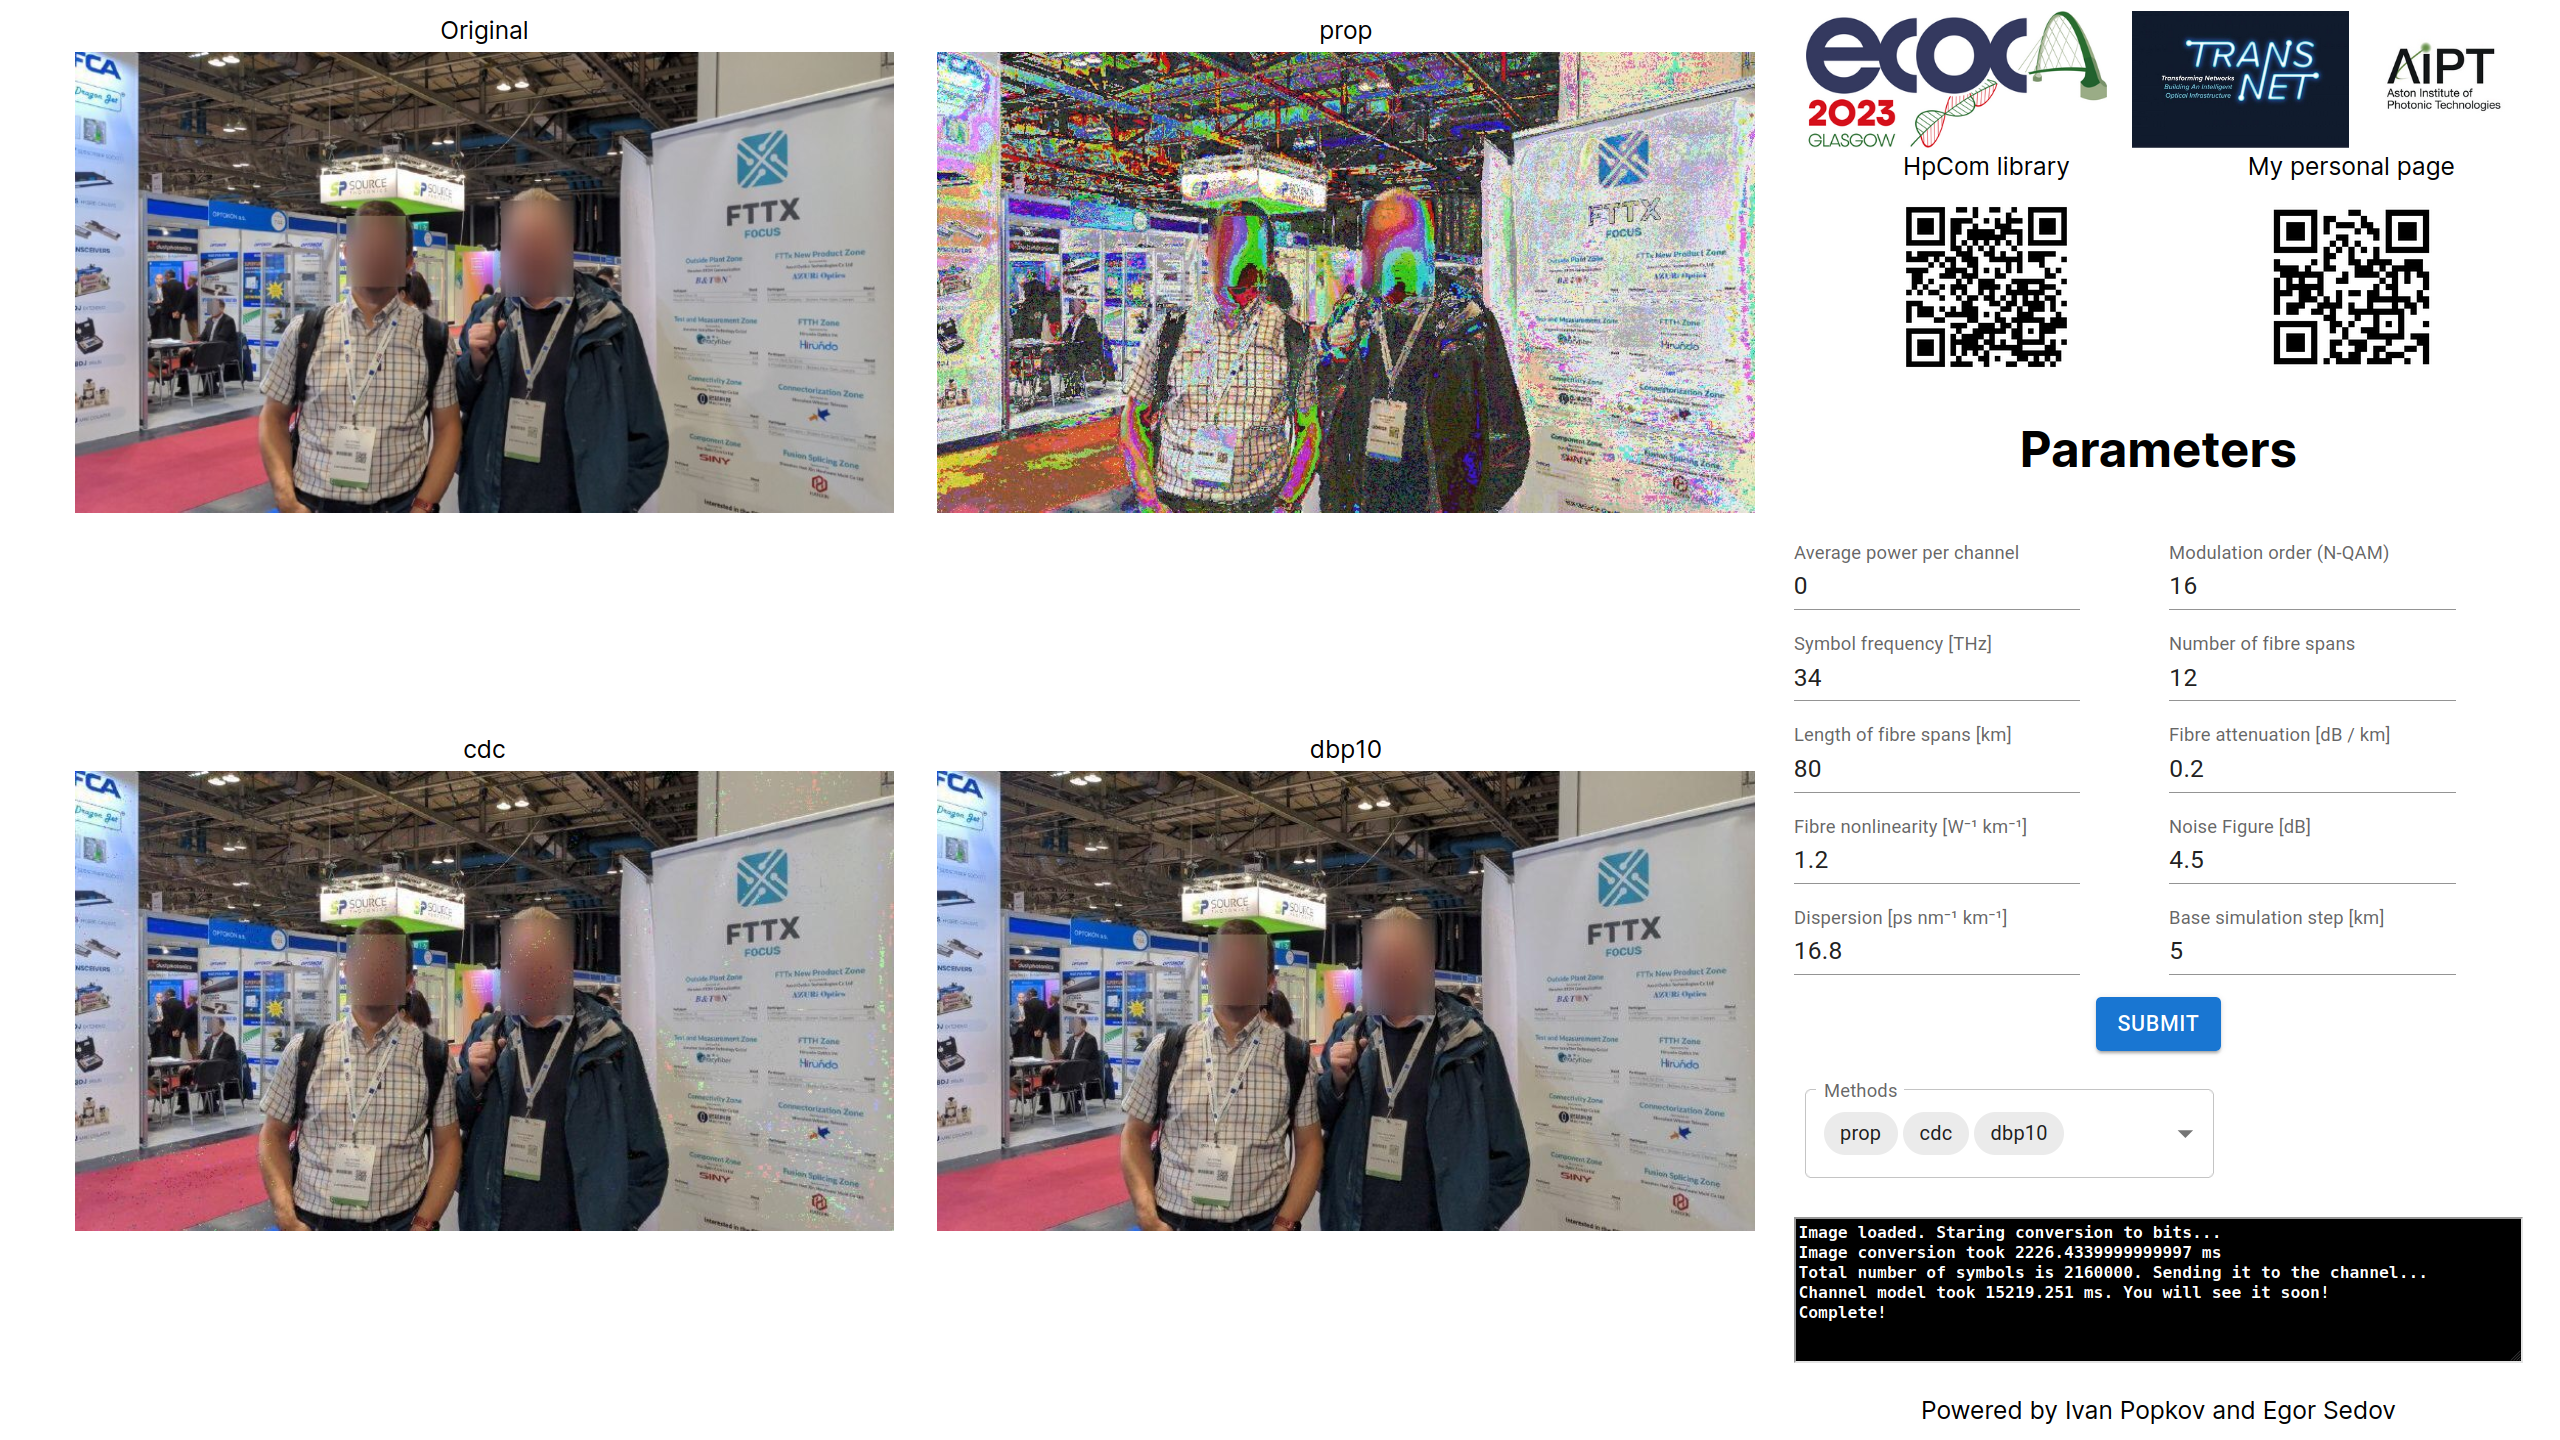
\includegraphics[width=\linewidth]{images/demo/demo1.png}
    \caption{ECOC2023 GLASGOW Demo Interface: Left side displays 4 spans for image selection, while the right side offers sections for simulation parameter adjustments, mode selection, and a log console.}
    \label{fig:demo1}
\end{figure}
\end{landscape}

\begin{landscape}
\begin{figure}[htpb]
    \begin{minipage}[h]{0.55\linewidth}
        \begin{minipage}[h]{0.49\linewidth}
        \center{
            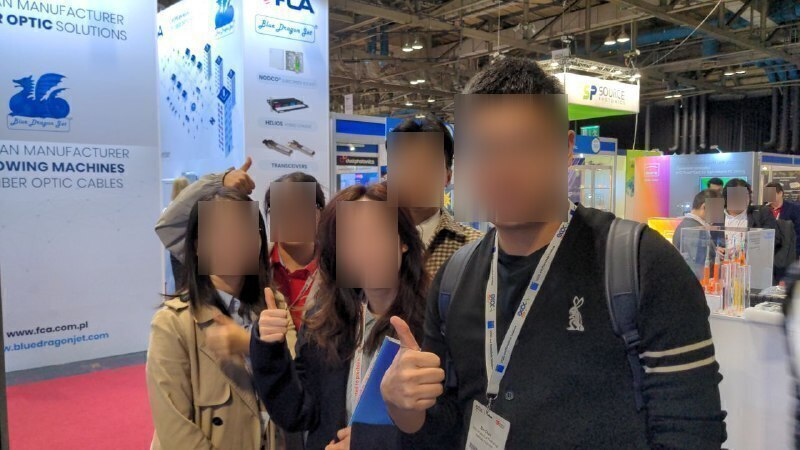
\includegraphics[width=1\linewidth]{images/demo/twc/twc_0.jpg} (a) \\
        }
        \end{minipage}
        \hfill
        \begin{minipage}[h]{0.49\linewidth}
        \center{
            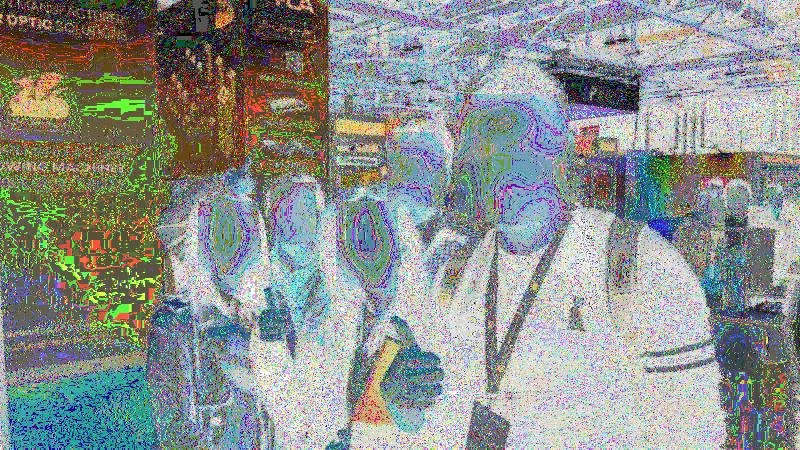
\includegraphics[width=1\linewidth]{images/demo/twc/twc_10.jpg} (b) \\
        }
        \end{minipage}
        
        \begin{minipage}[h]{0.49\linewidth}
        \center{
            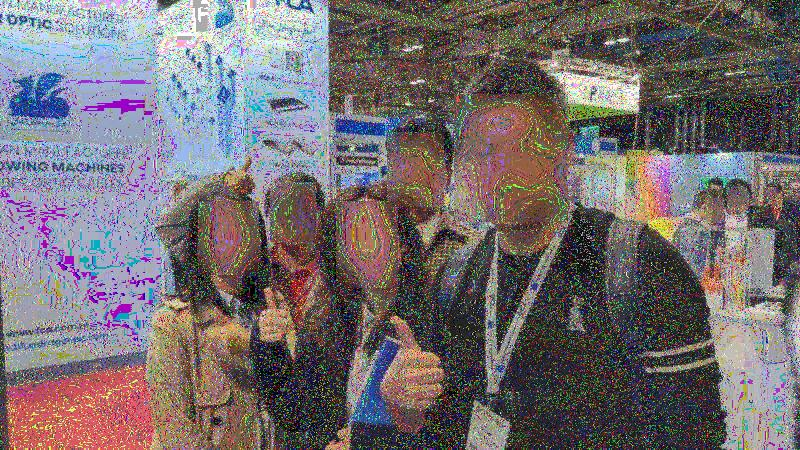
\includegraphics[width=1\linewidth]{images/demo/twc/twc_1.jpg} (c) \\
        }
        \end{minipage}
        \hfill
        \begin{minipage}[h]{0.49\linewidth}
        \center{
            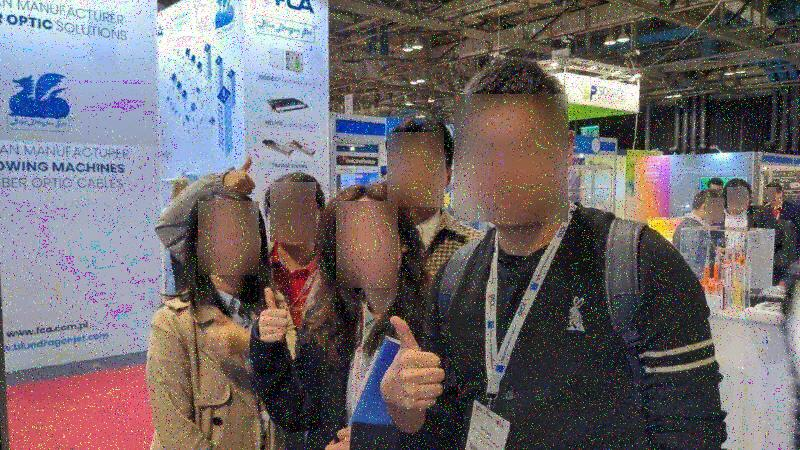
\includegraphics[width=1\linewidth]{images/demo/twc/twc_2.jpg} (d) \\
        }
        \end{minipage}
        
        \begin{minipage}[h]{0.49\linewidth}
        \center{
            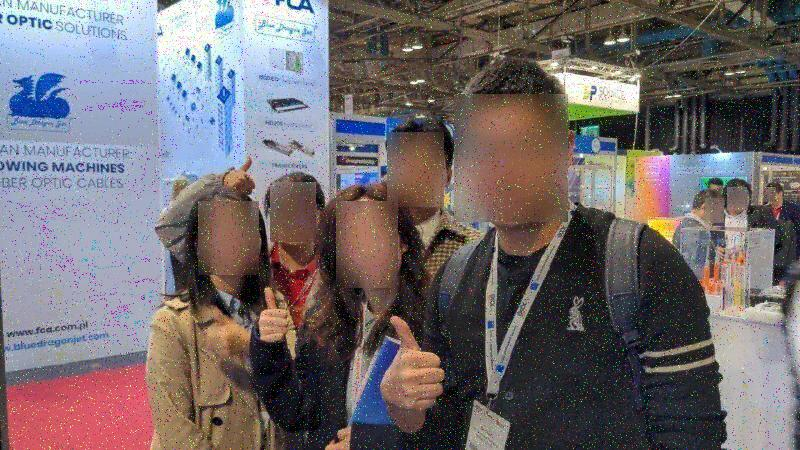
\includegraphics[width=1\linewidth]{images/demo/twc/twc_3.jpg} (e) \\
        }
        \end{minipage}
        \hfill
        \begin{minipage}[h]{0.49\linewidth}
        \center{
            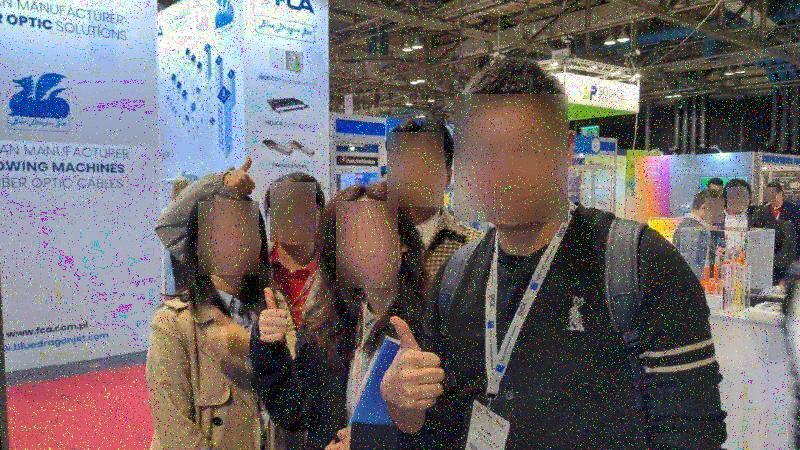
\includegraphics[width=1\linewidth]{images/demo/twc/twc_5.jpg} (f) \\
        }
        \end{minipage}
    \end{minipage}
    \hfill
    \begin{minipage}[h]{0.45\linewidth}
        \begin{minipage}[h]{0.49\linewidth}
        \center{
            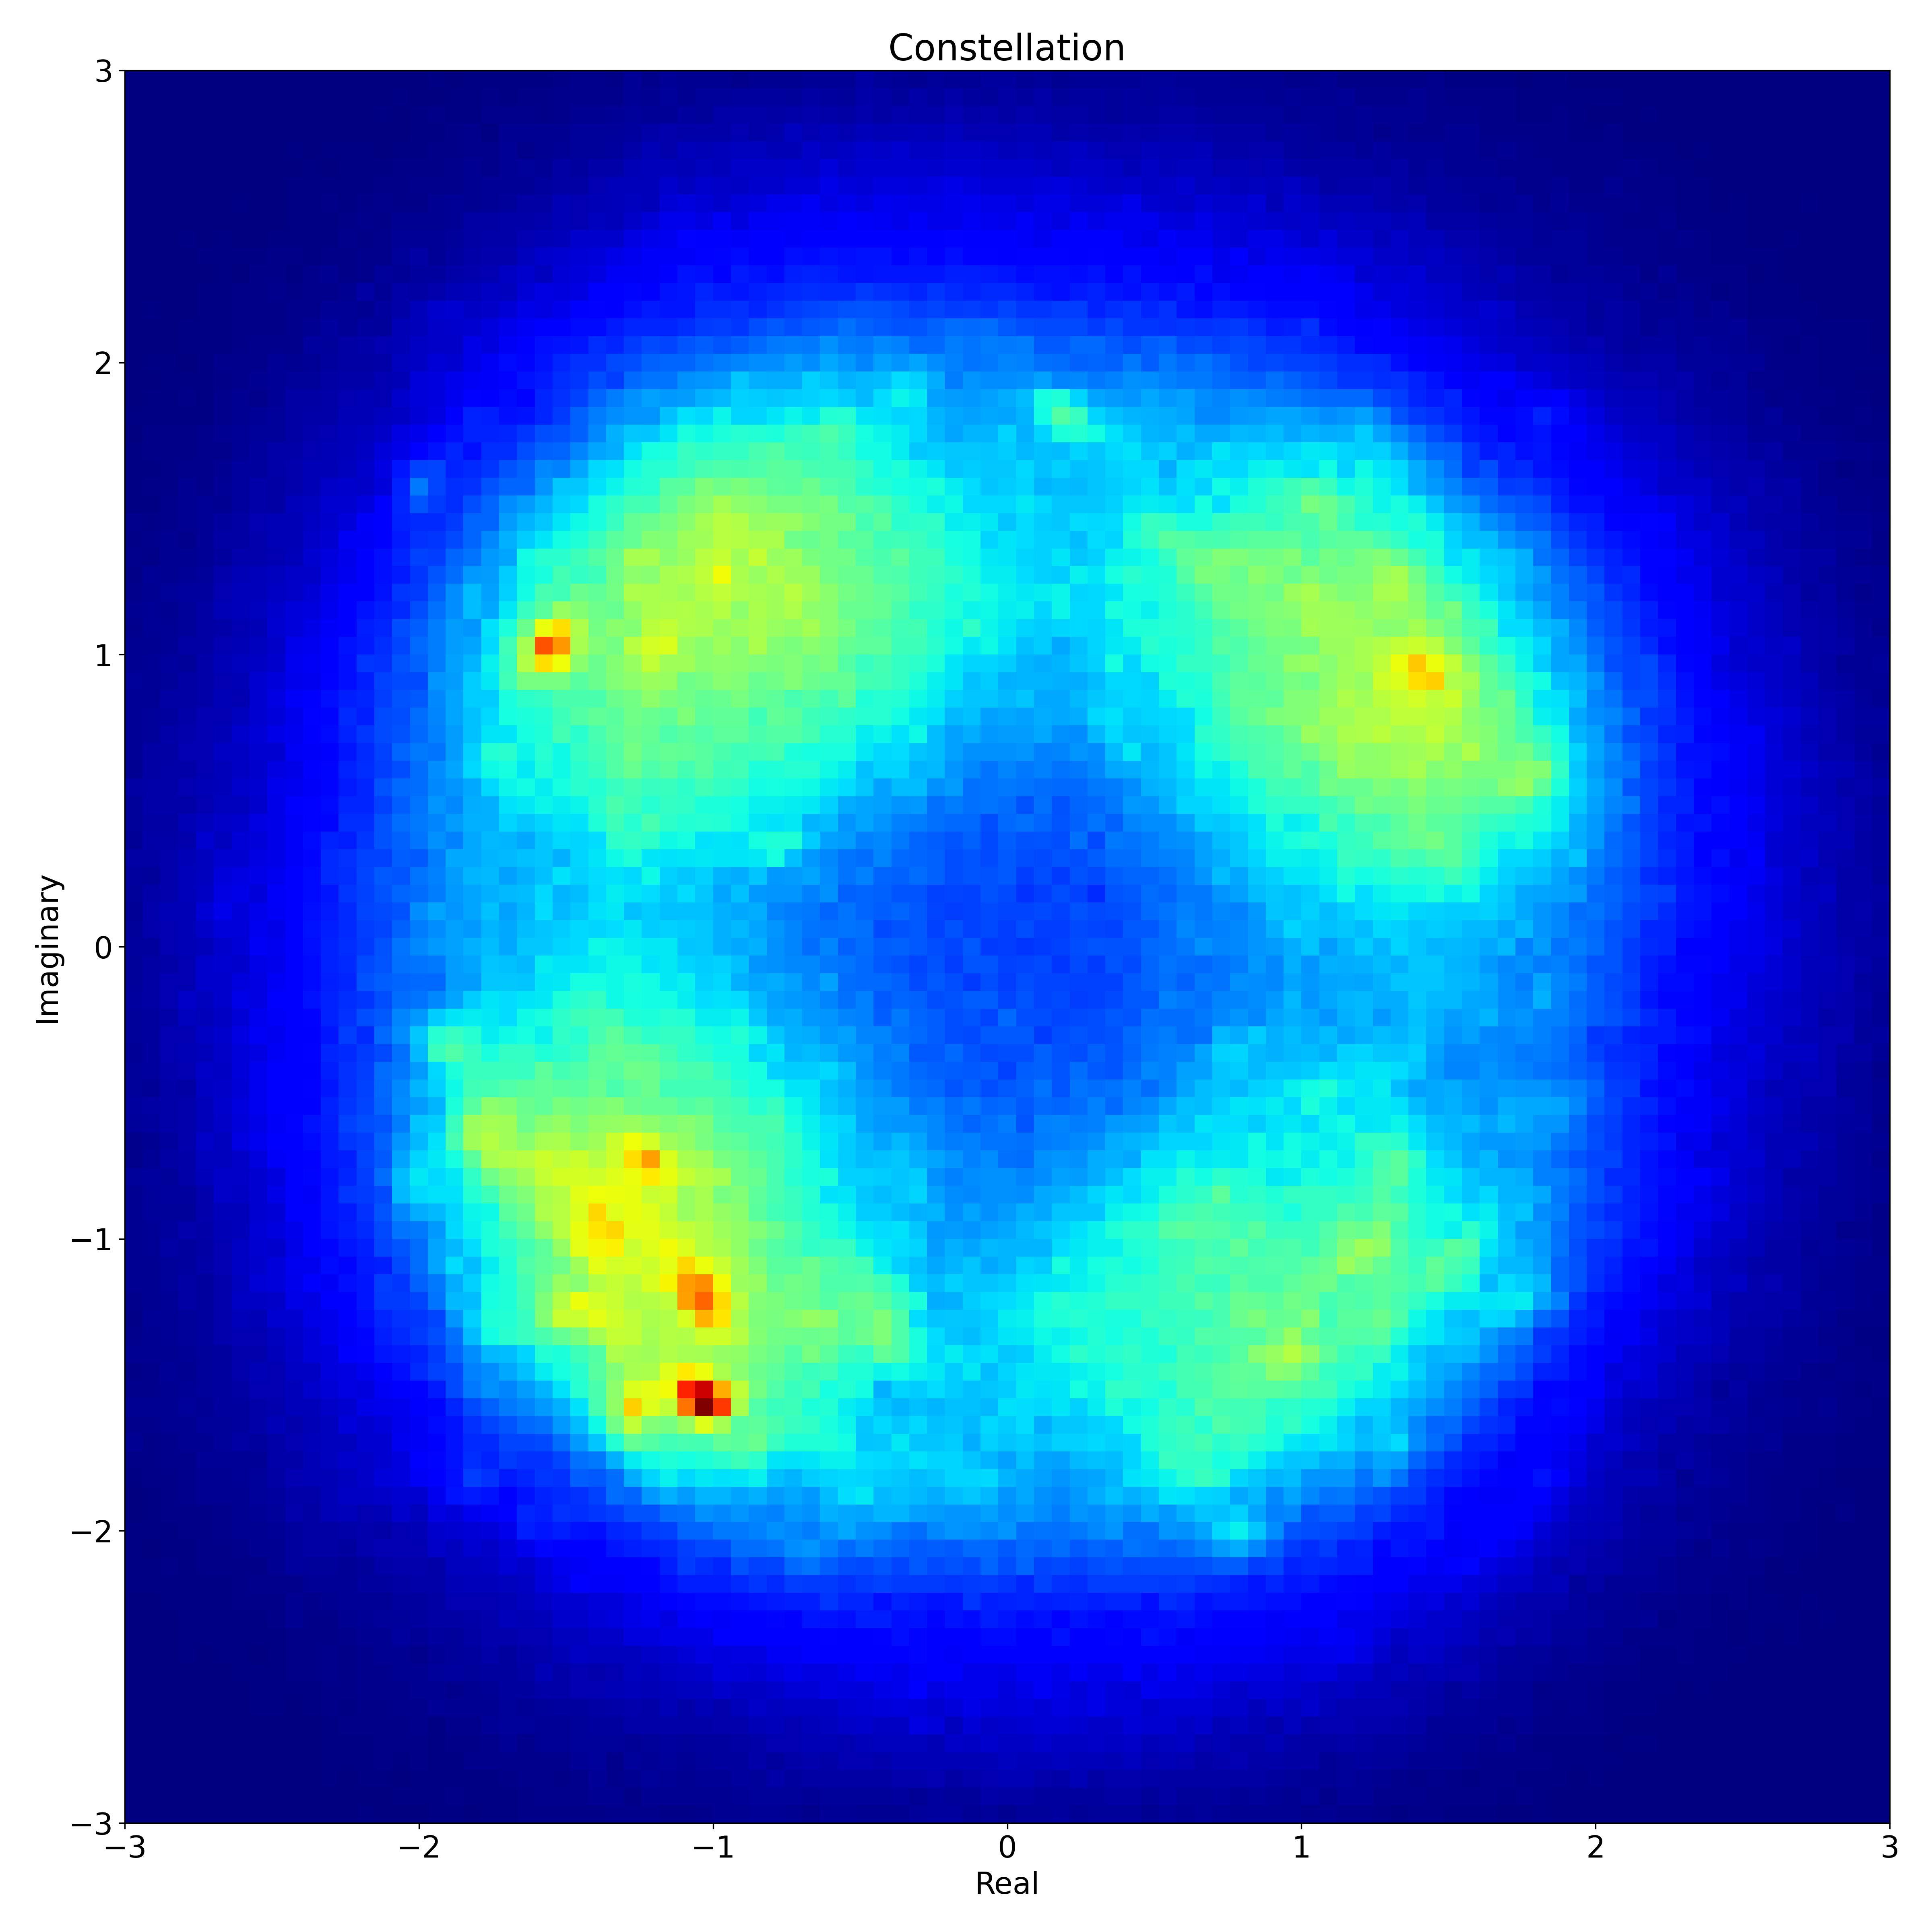
\includegraphics[width=1\linewidth]{images/demo/twc/twc_6.jpg} (g) \\
        }
        \end{minipage}
        \hfill
        \begin{minipage}[h]{0.49\linewidth}
        \center{
            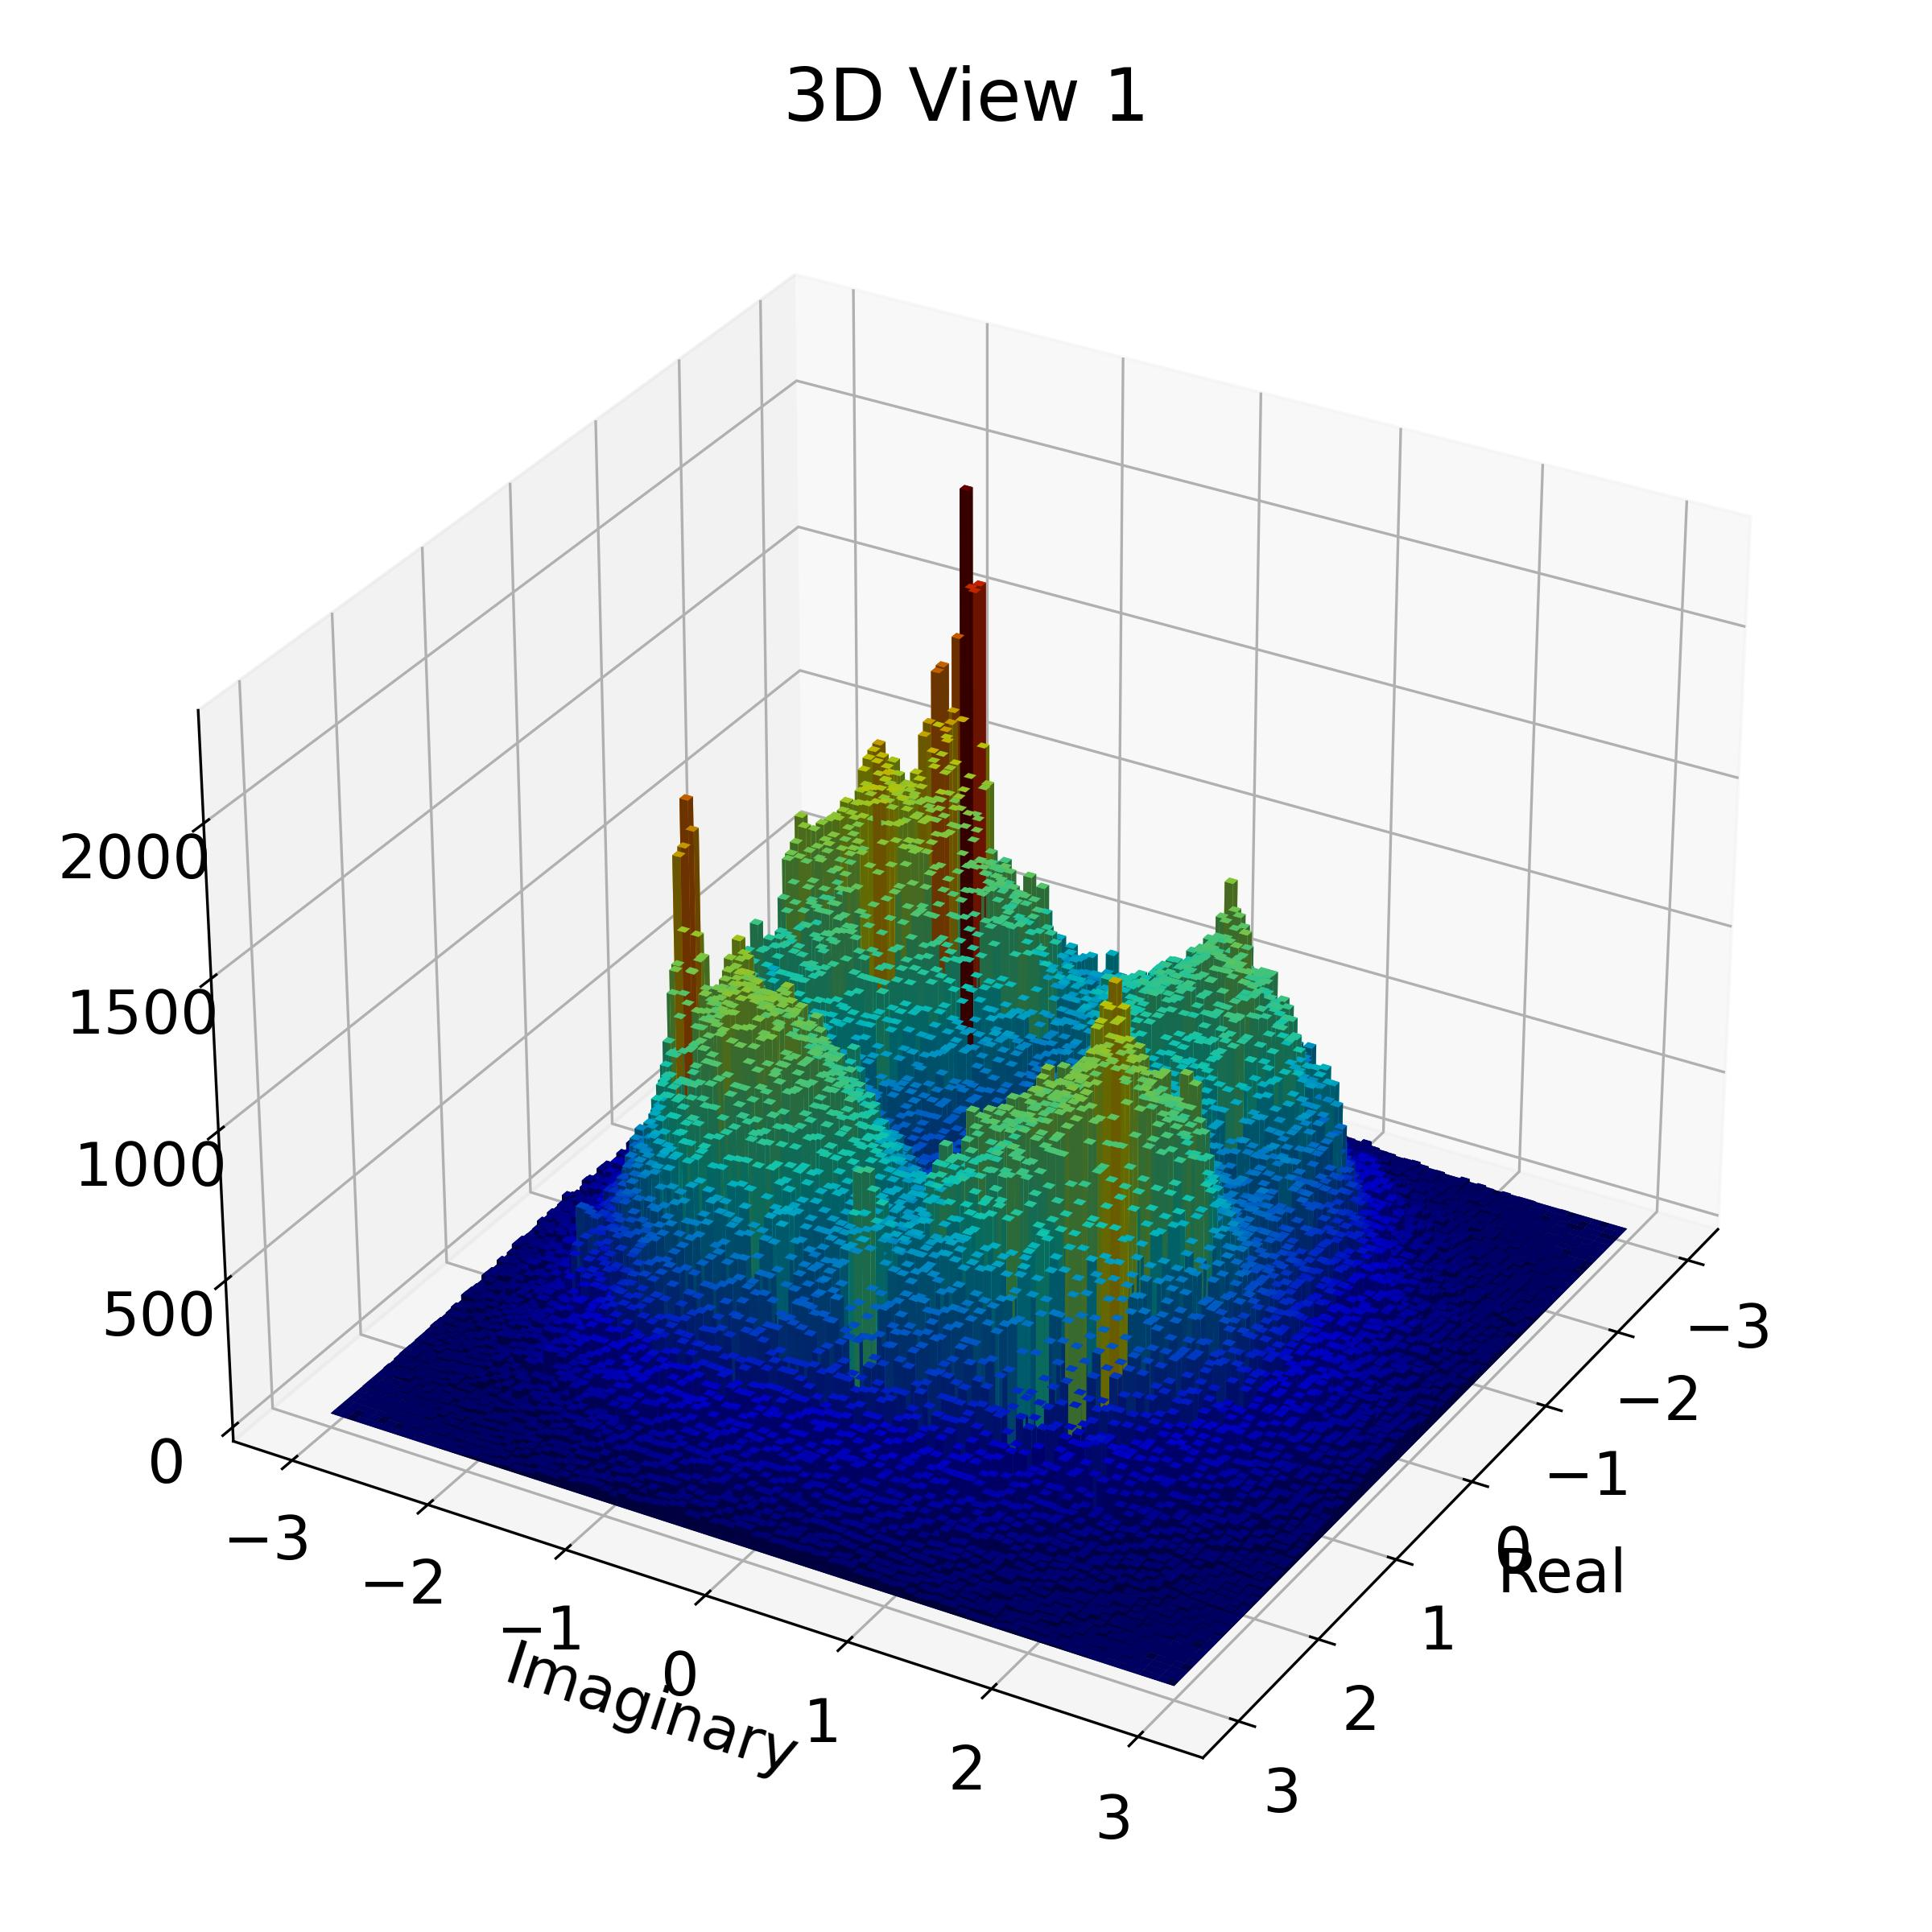
\includegraphics[width=1\linewidth]{images/demo/twc/twc_7.jpg} (h) \\
        }
        \end{minipage}
        \vfill
        \begin{minipage}[h]{0.49\linewidth}
        \center{
            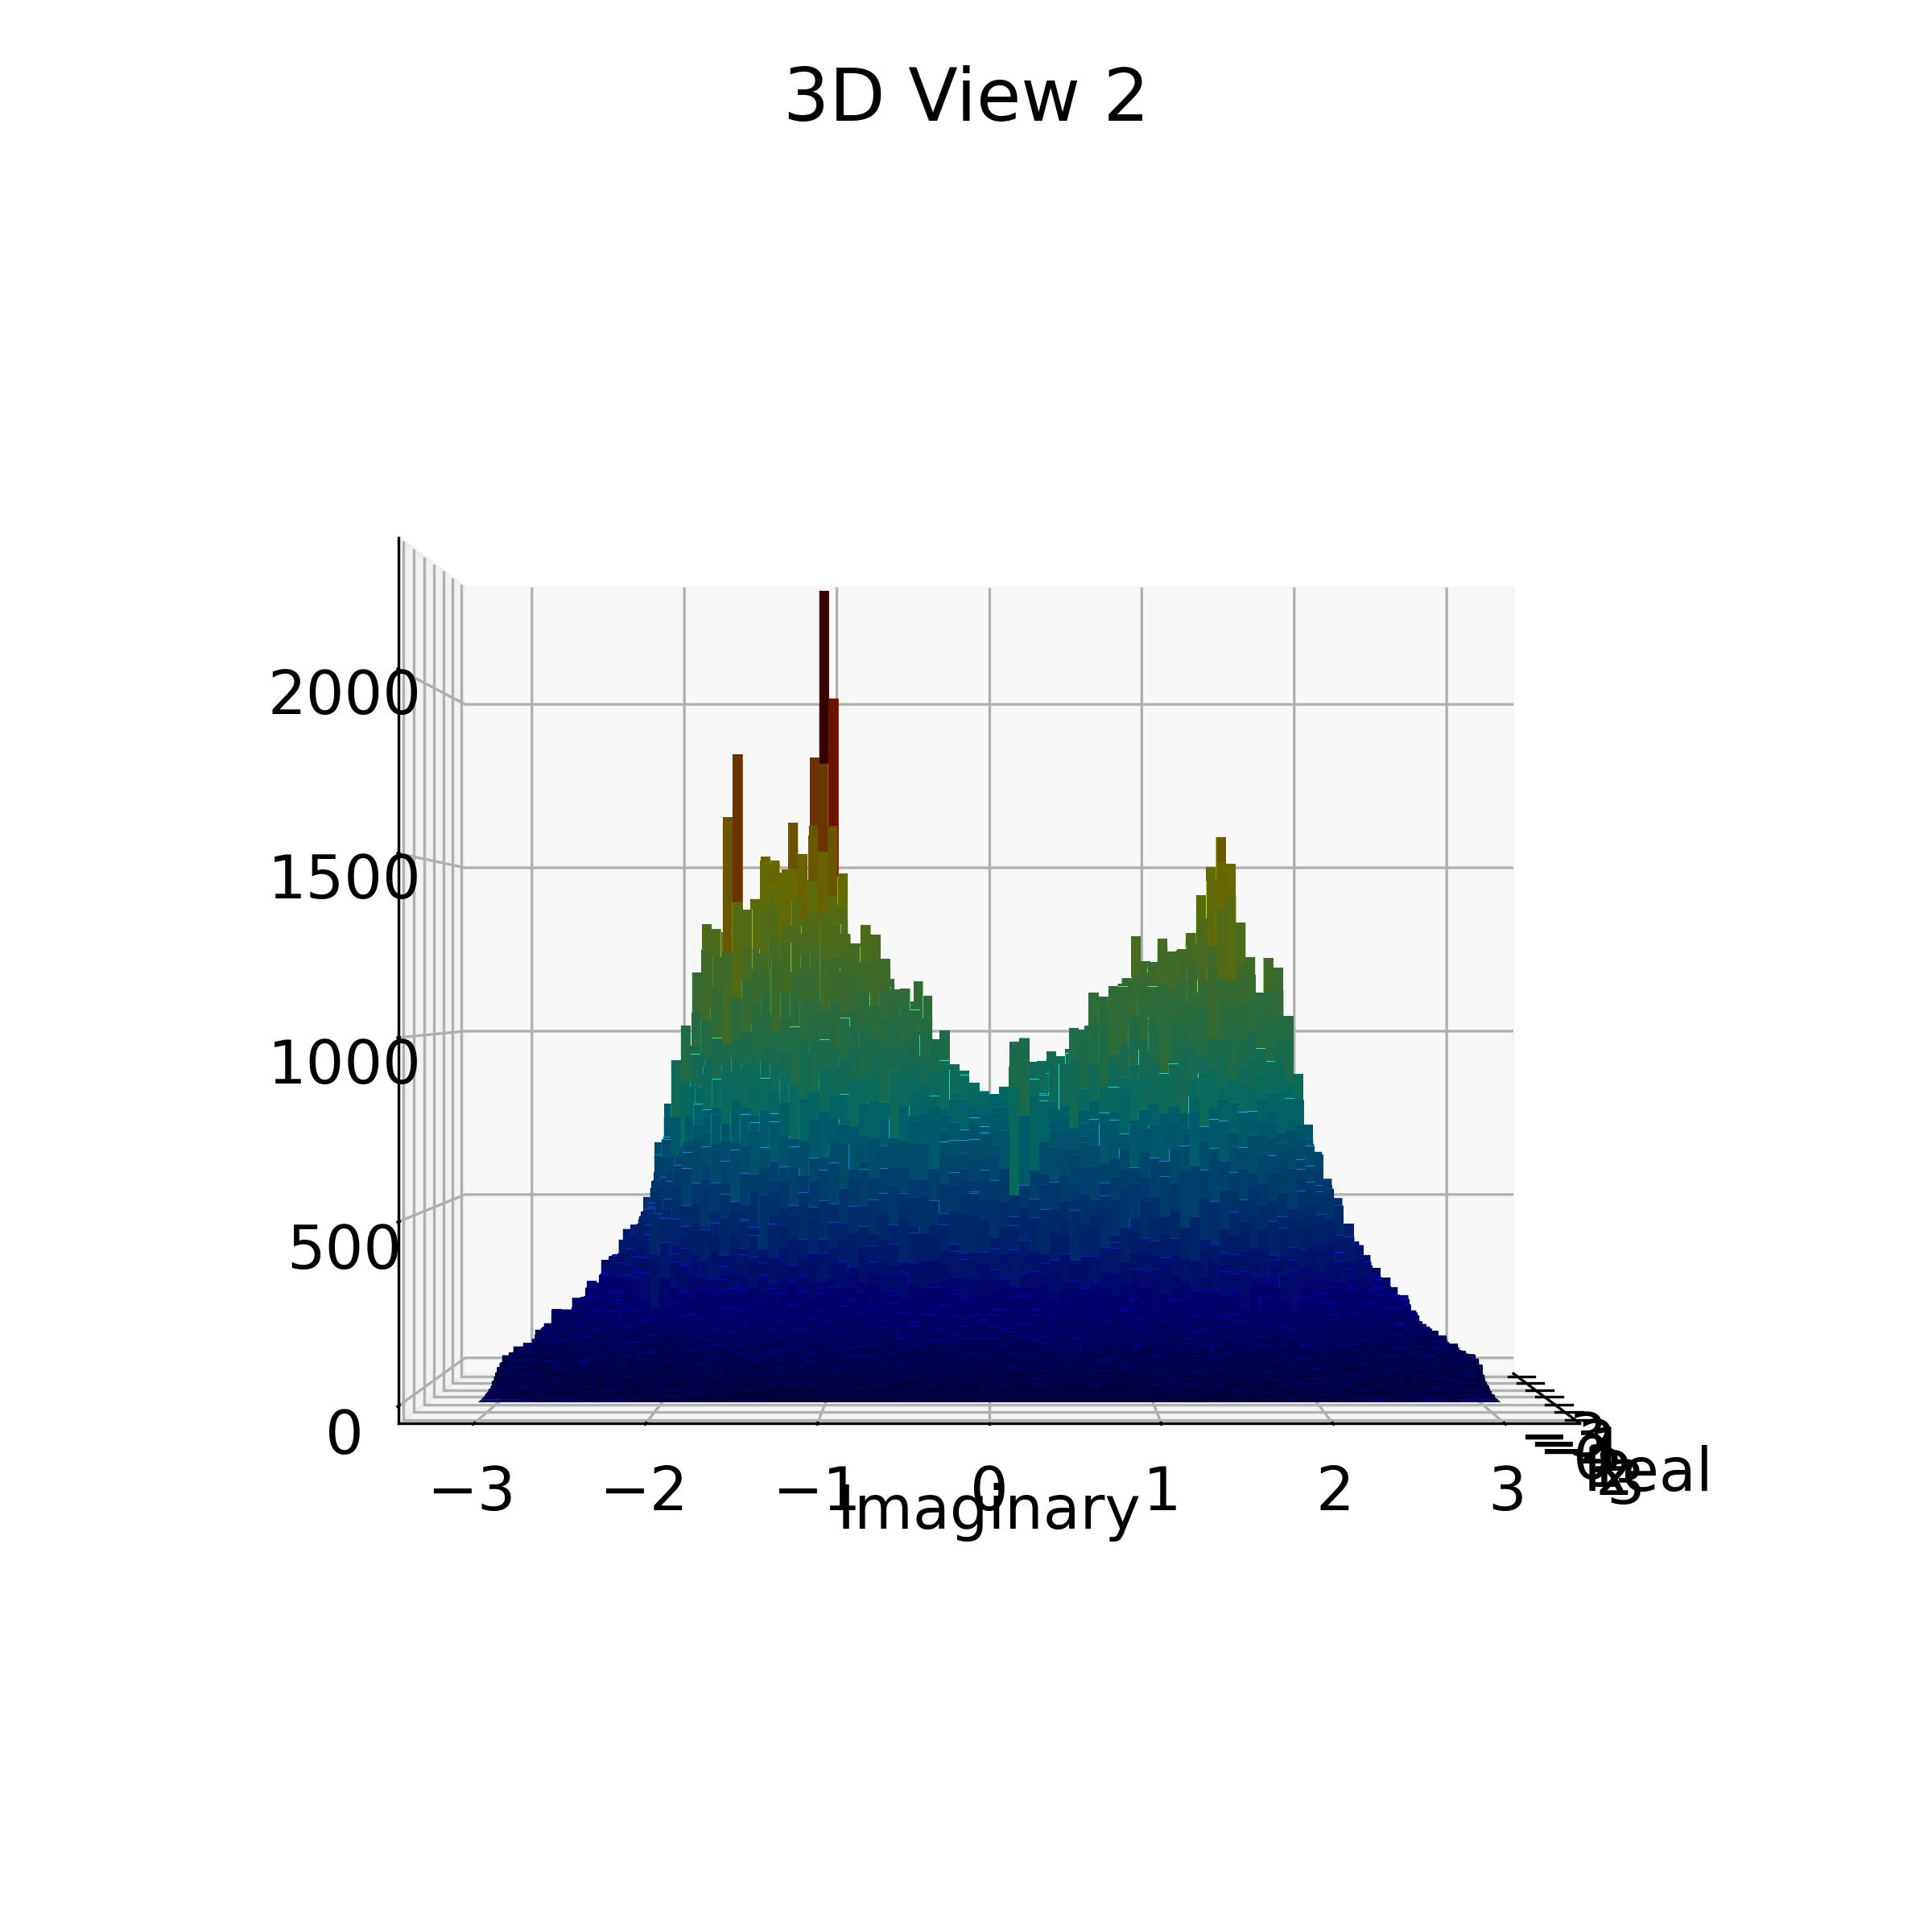
\includegraphics[width=1\linewidth]{images/demo/twc/twc_8.jpg} (i) \\
        }
        \end{minipage}
        \hfill
        \begin{minipage}[h]{0.49\linewidth}
        \center{
            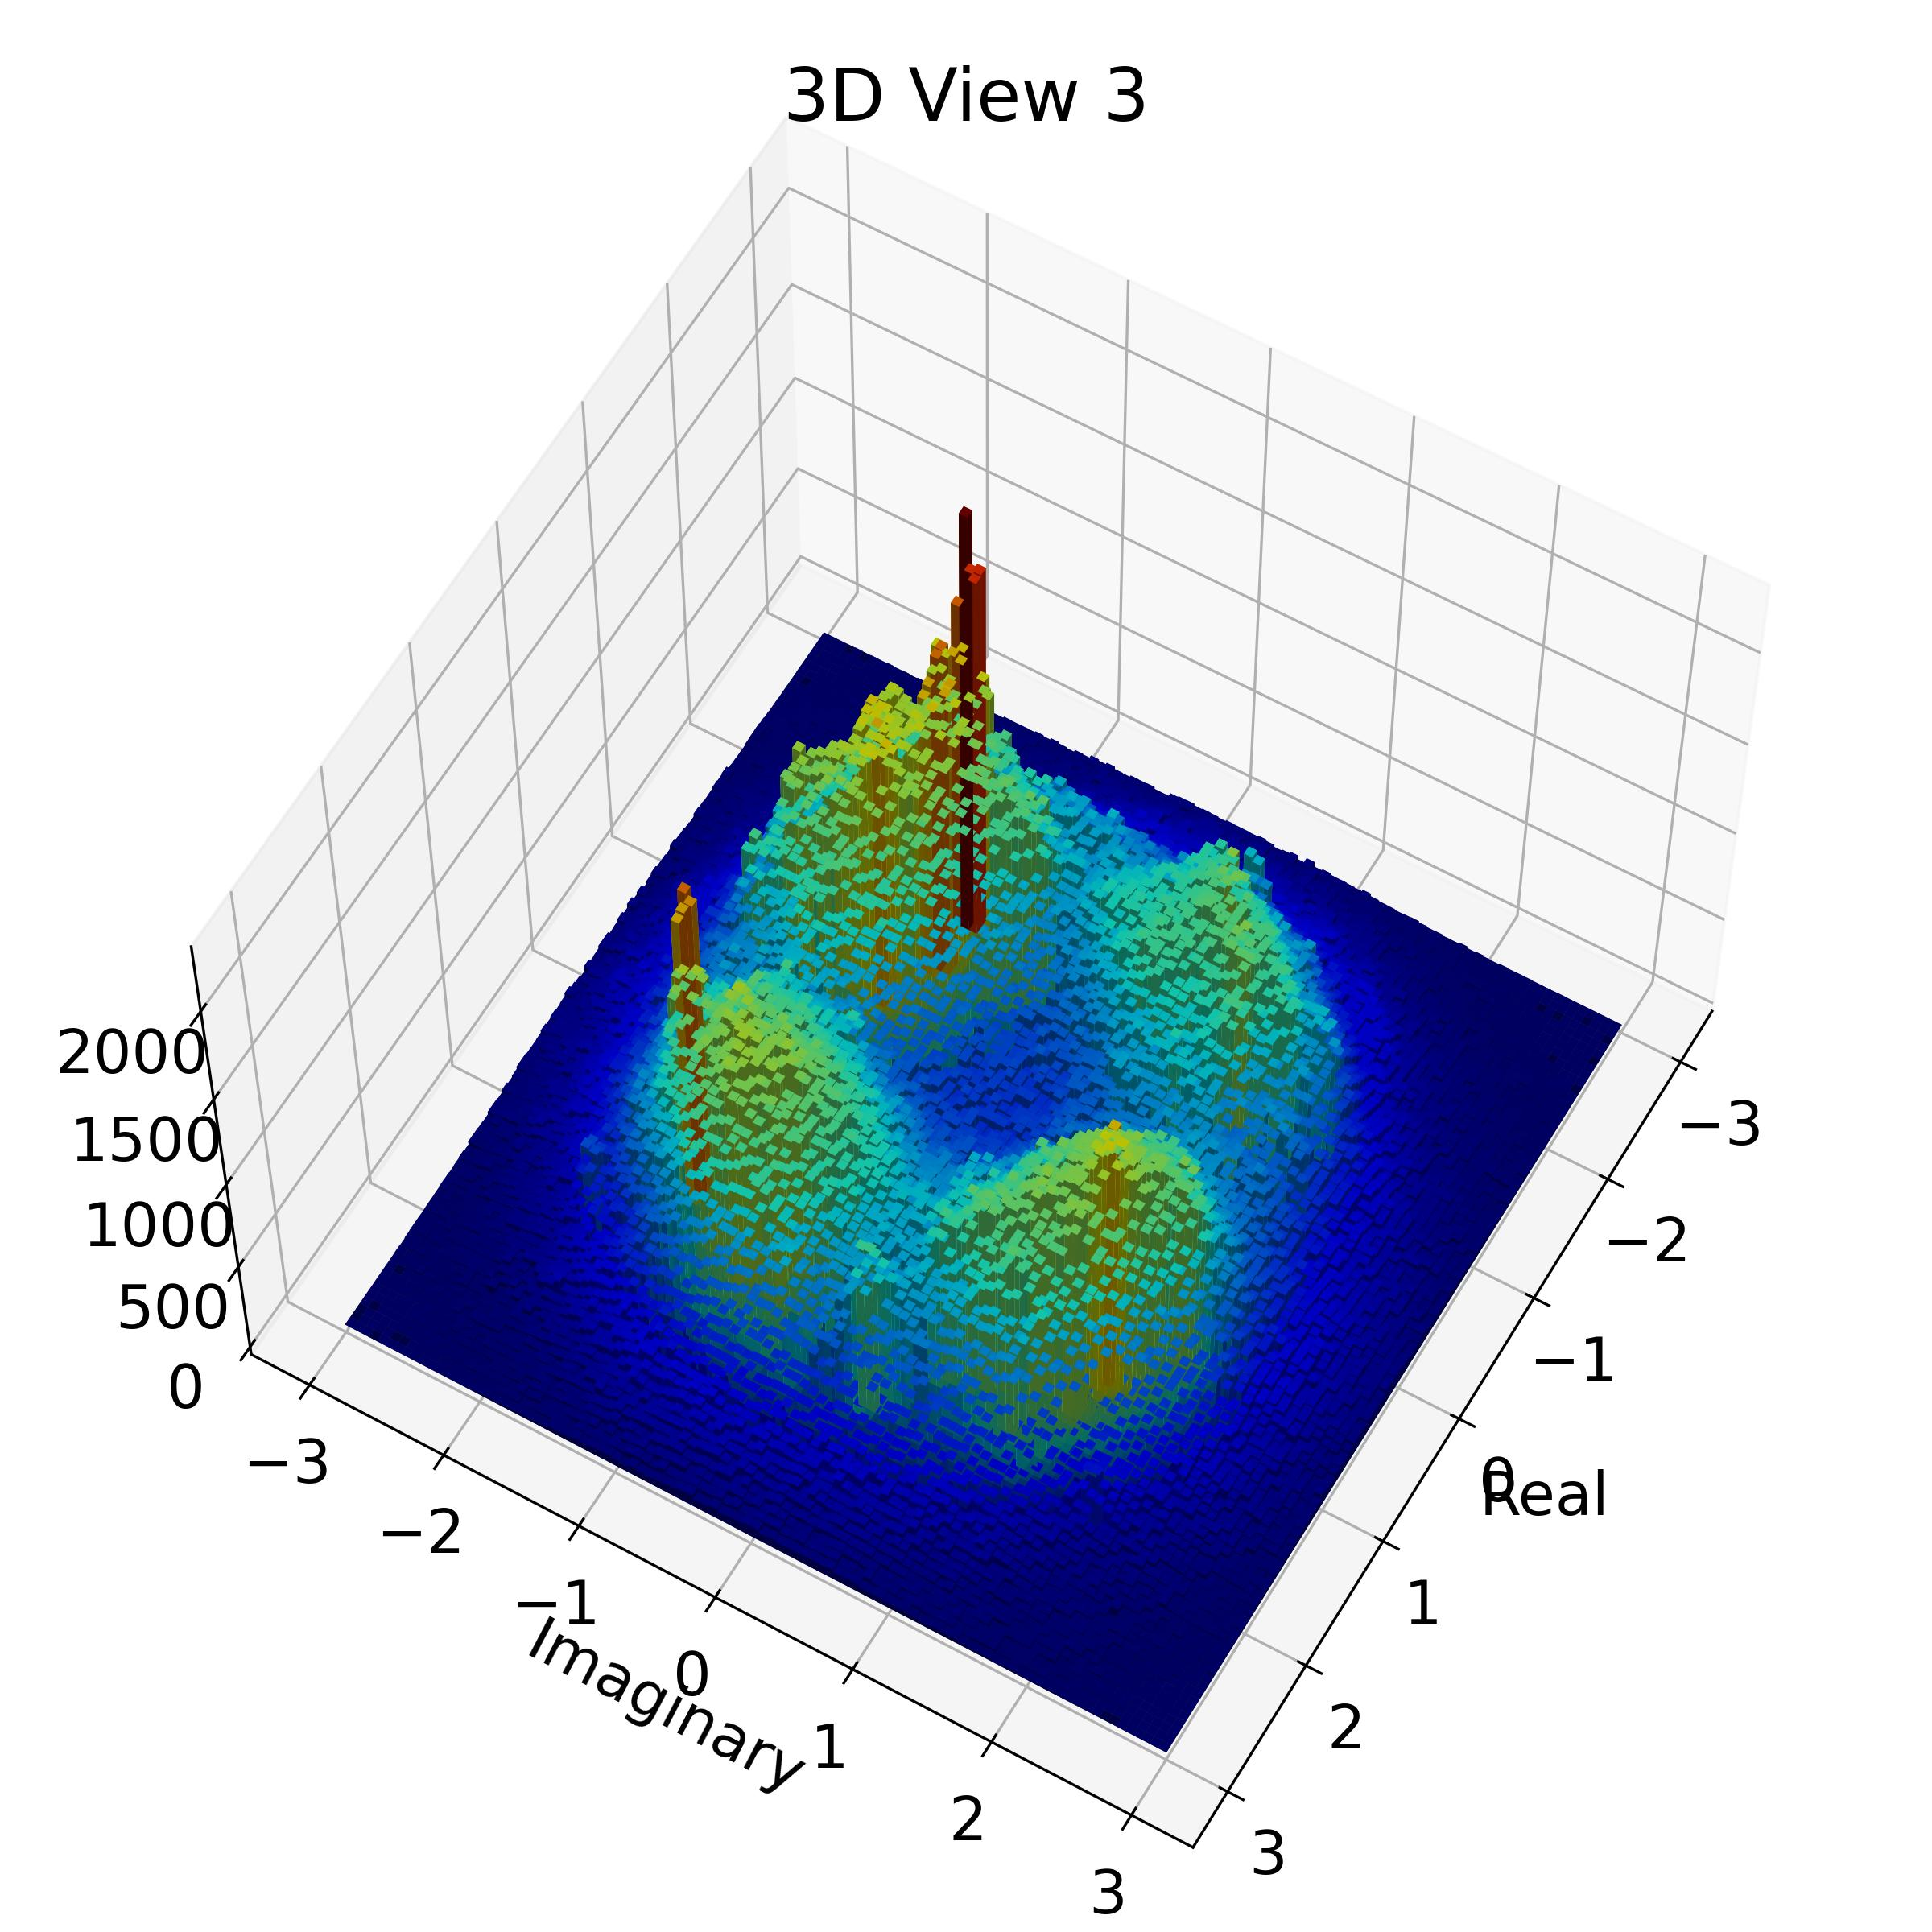
\includegraphics[width=1\linewidth]{images/demo/twc/twc_9.jpg} (j)
        }
        \end{minipage}
    \end{minipage}
    \caption{Signal propagation with parameters: $10 \times 50$ $[\textrm{km}]$ spans of \gls{twc} fibre, attenuation coefficient of $\alpha = 0.2$ $[\textrm{dB}/\textrm{km}]$, EDFA noise figure 4.5 \textrm{[dB]}, a dispersion coefficient of $D = 2.8$ $\textrm{ps}/[\textrm{nm} \cdot \textrm{km}]$, and a nonlinear coefficient of $\gamma = 2.5$ $[\textrm{W} \cdot \textrm{km}]^{-1}$, average signal power $P_{ave} = 5$ $\textrm{dBm}$, \gls{qpsk} format. \textbf{(a)} Original image. \textbf{(b)} Image post-propagation without equalisation. \textbf{(c)} Image after \gls{cdc} and \gls{npe}. \textbf{(d)} and \textbf{(e)} \gls{dbp} with 2 and 3 steps per span, respectively. \textbf{(f)} Image after \gls{nn} equalisation for received symbols. \textbf{(g)} to \textbf{(j)} Various constellation diagram representations.}
    \label{fig:demo_twc}
\end{figure}
\end{landscape}

\begin{landscape}
\begin{figure}[htpb]
    \begin{minipage}[h]{0.55\linewidth}
        \begin{minipage}[h]{0.49\linewidth}
        \center{
            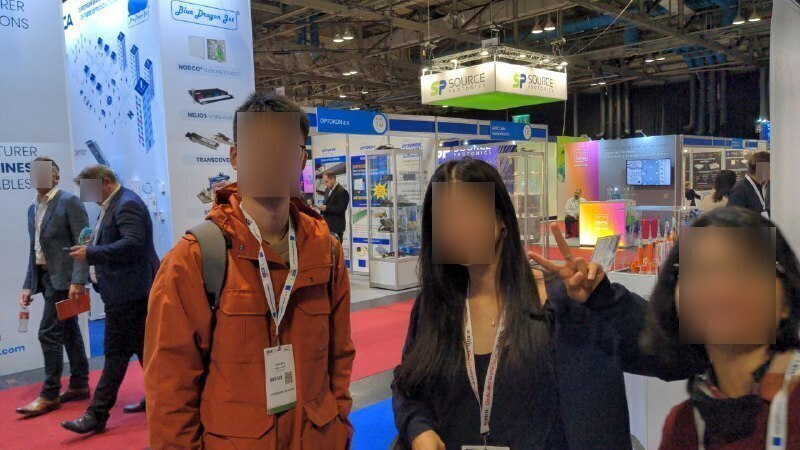
\includegraphics[width=1\linewidth]{images/demo/smf/smf_0.jpg} (a) \\
        }
        \end{minipage}
        \hfill
        \begin{minipage}[h]{0.49\linewidth}
        \center{
            
\includegraphics[width=1\linewidth]{images/demo/smf/smf_10.jpg} (b) \\
        }
        \end{minipage}
        
        \begin{minipage}[h]{0.49\linewidth}
        \center{
            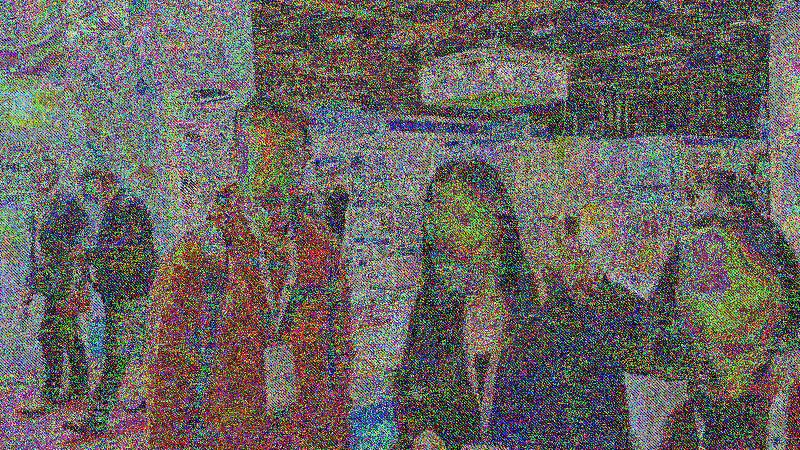
\includegraphics[width=1\linewidth]{images/demo/smf/smf_1.jpg} (c) \\
        }
        \end{minipage}
        \hfill
        \begin{minipage}[h]{0.49\linewidth}
        \center{
            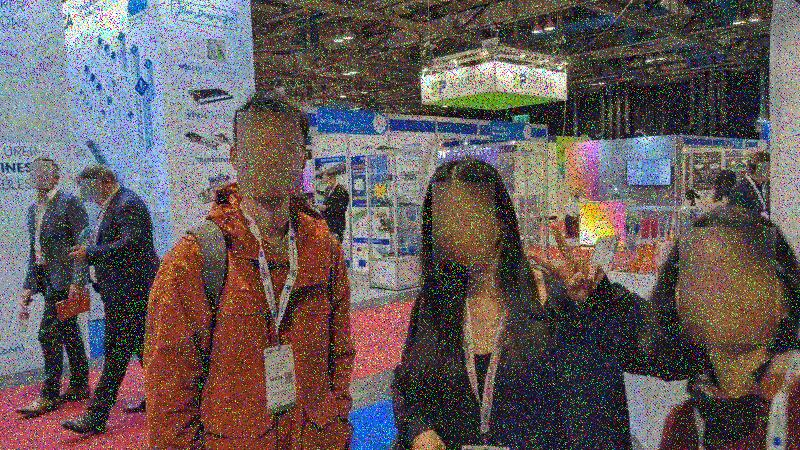
\includegraphics[width=1\linewidth]{images/demo/smf/smf_2.jpg} (d) \\
        }
        \end{minipage}
        
        \begin{minipage}[h]{0.49\linewidth}
        \center{
            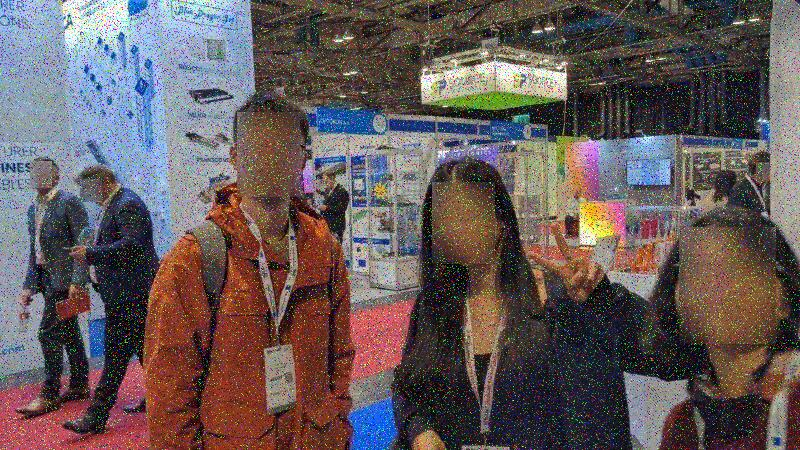
\includegraphics[width=1\linewidth]{images/demo/smf/smf_3.jpg} (e) \\
        }
        \end{minipage}
        \hfill
        \begin{minipage}[h]{0.49\linewidth}
        \center{
            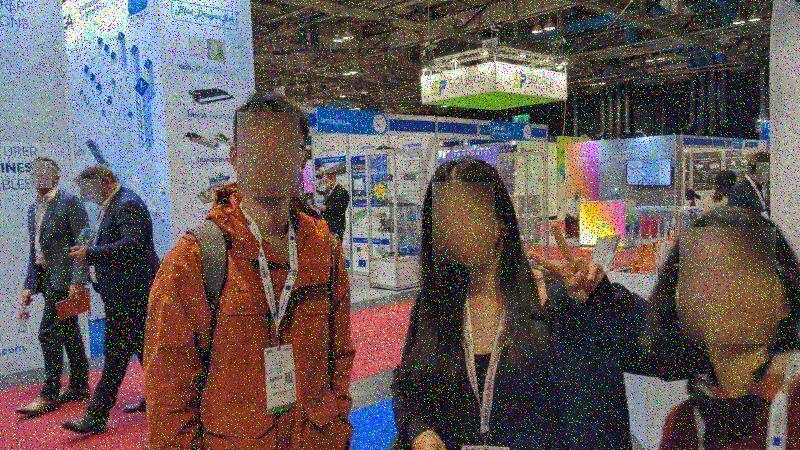
\includegraphics[width=1\linewidth]{images/demo/smf/smf_5.jpg} (f) \\
        }
        \end{minipage}
    \end{minipage}
    \hfill
    \begin{minipage}[h]{0.45\linewidth}
        \begin{minipage}[h]{0.49\linewidth}
        \center{
            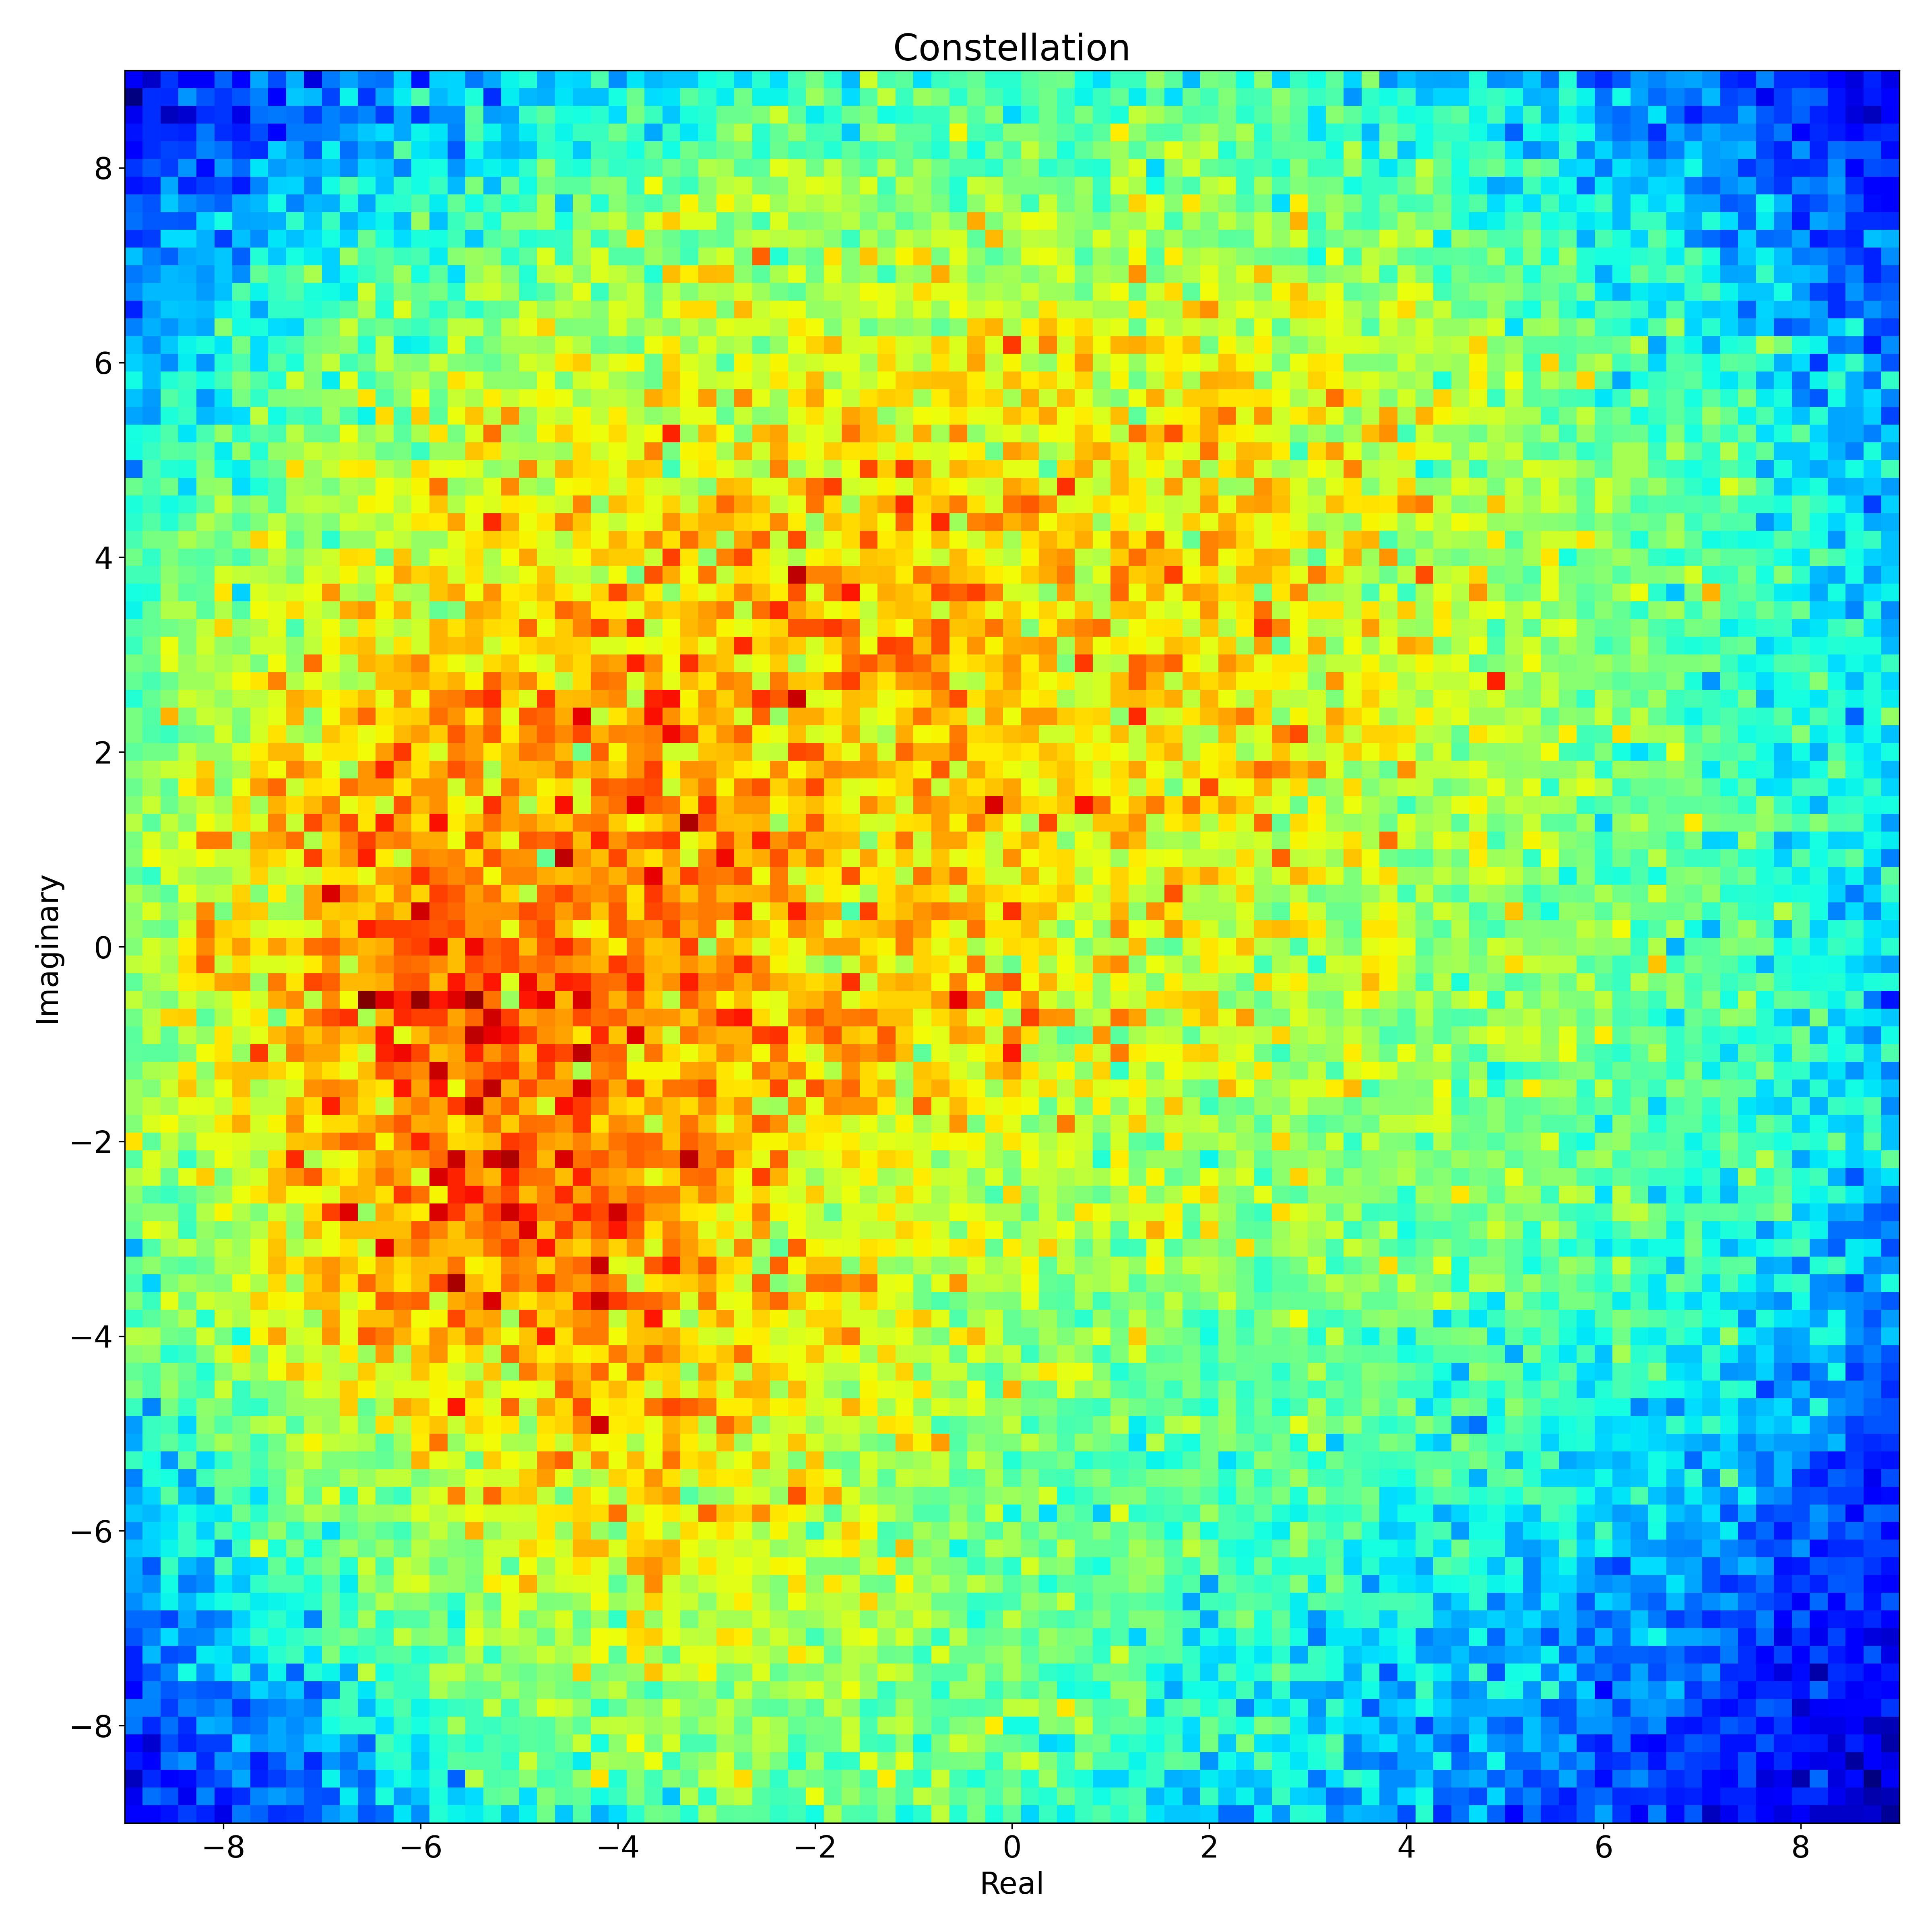
\includegraphics[width=1\linewidth]{images/demo/smf/smf_6.jpg} (g) \\
        }
        \end{minipage}
        \hfill
        \begin{minipage}[h]{0.49\linewidth}
        \center{
            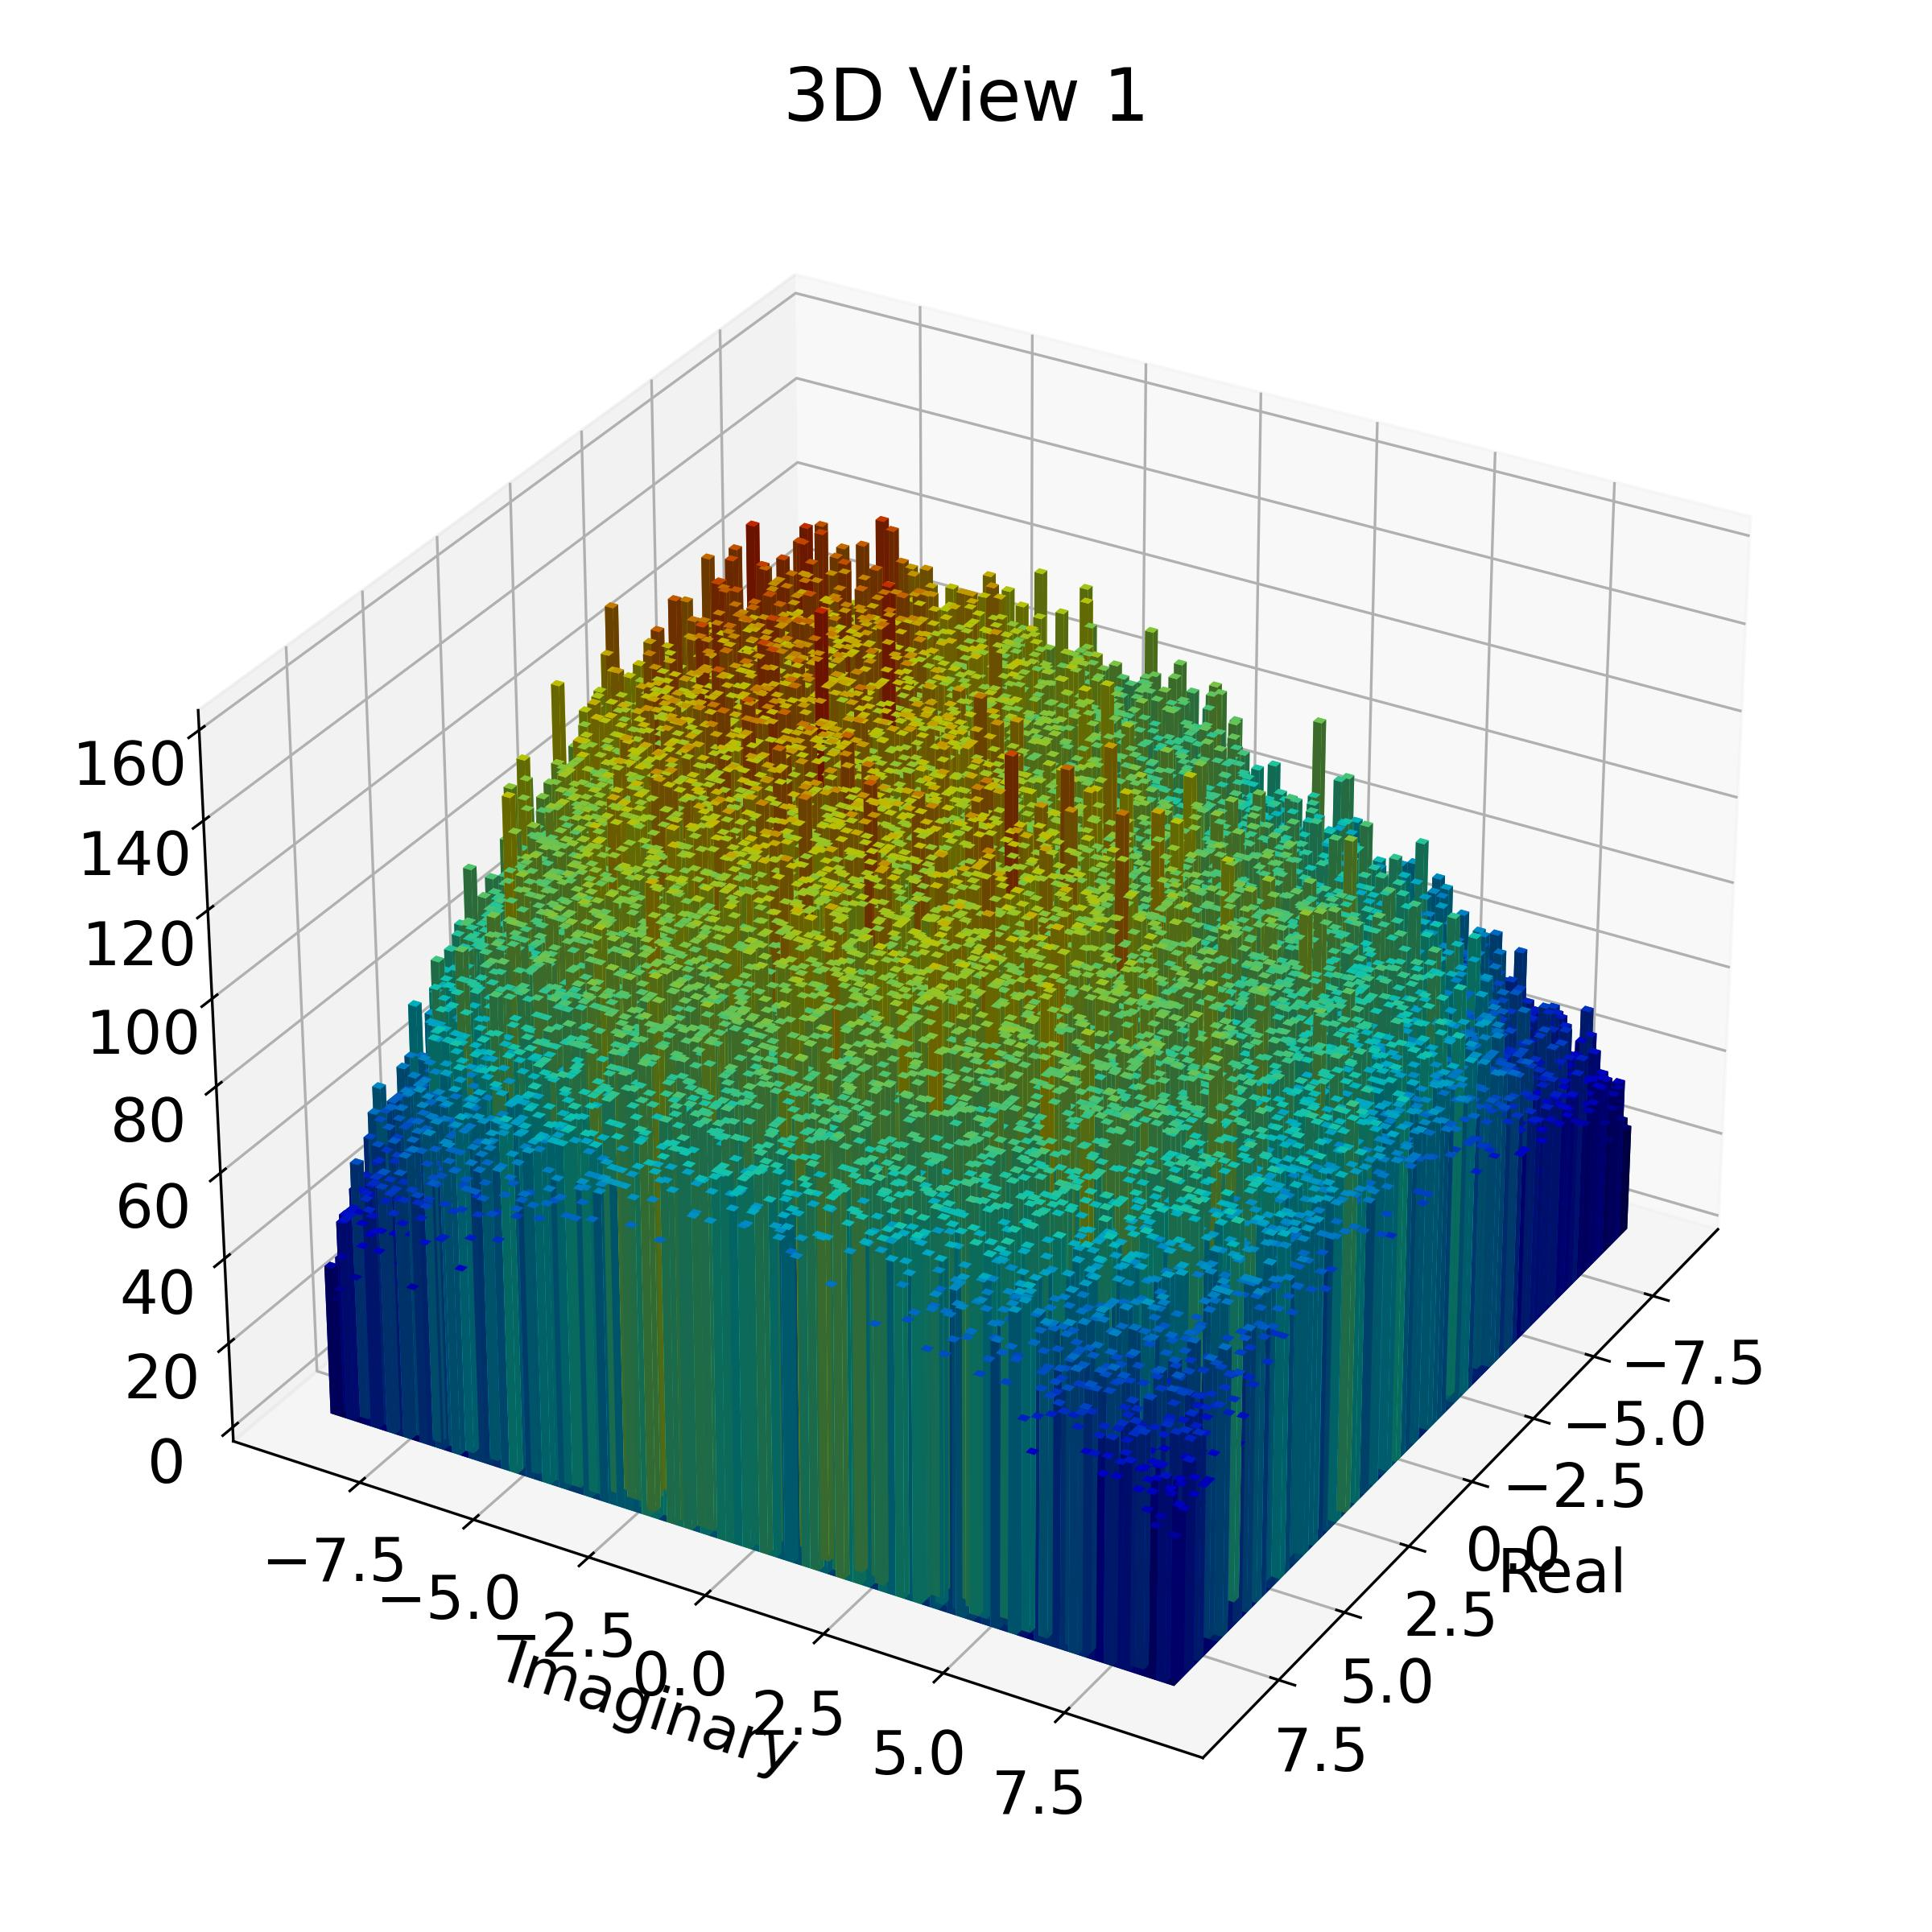
\includegraphics[width=1\linewidth]{images/demo/smf/smf_7.jpg} (h) \\
        }
        \end{minipage}
        \vfill
        \begin{minipage}[h]{0.49\linewidth}
        \center{
            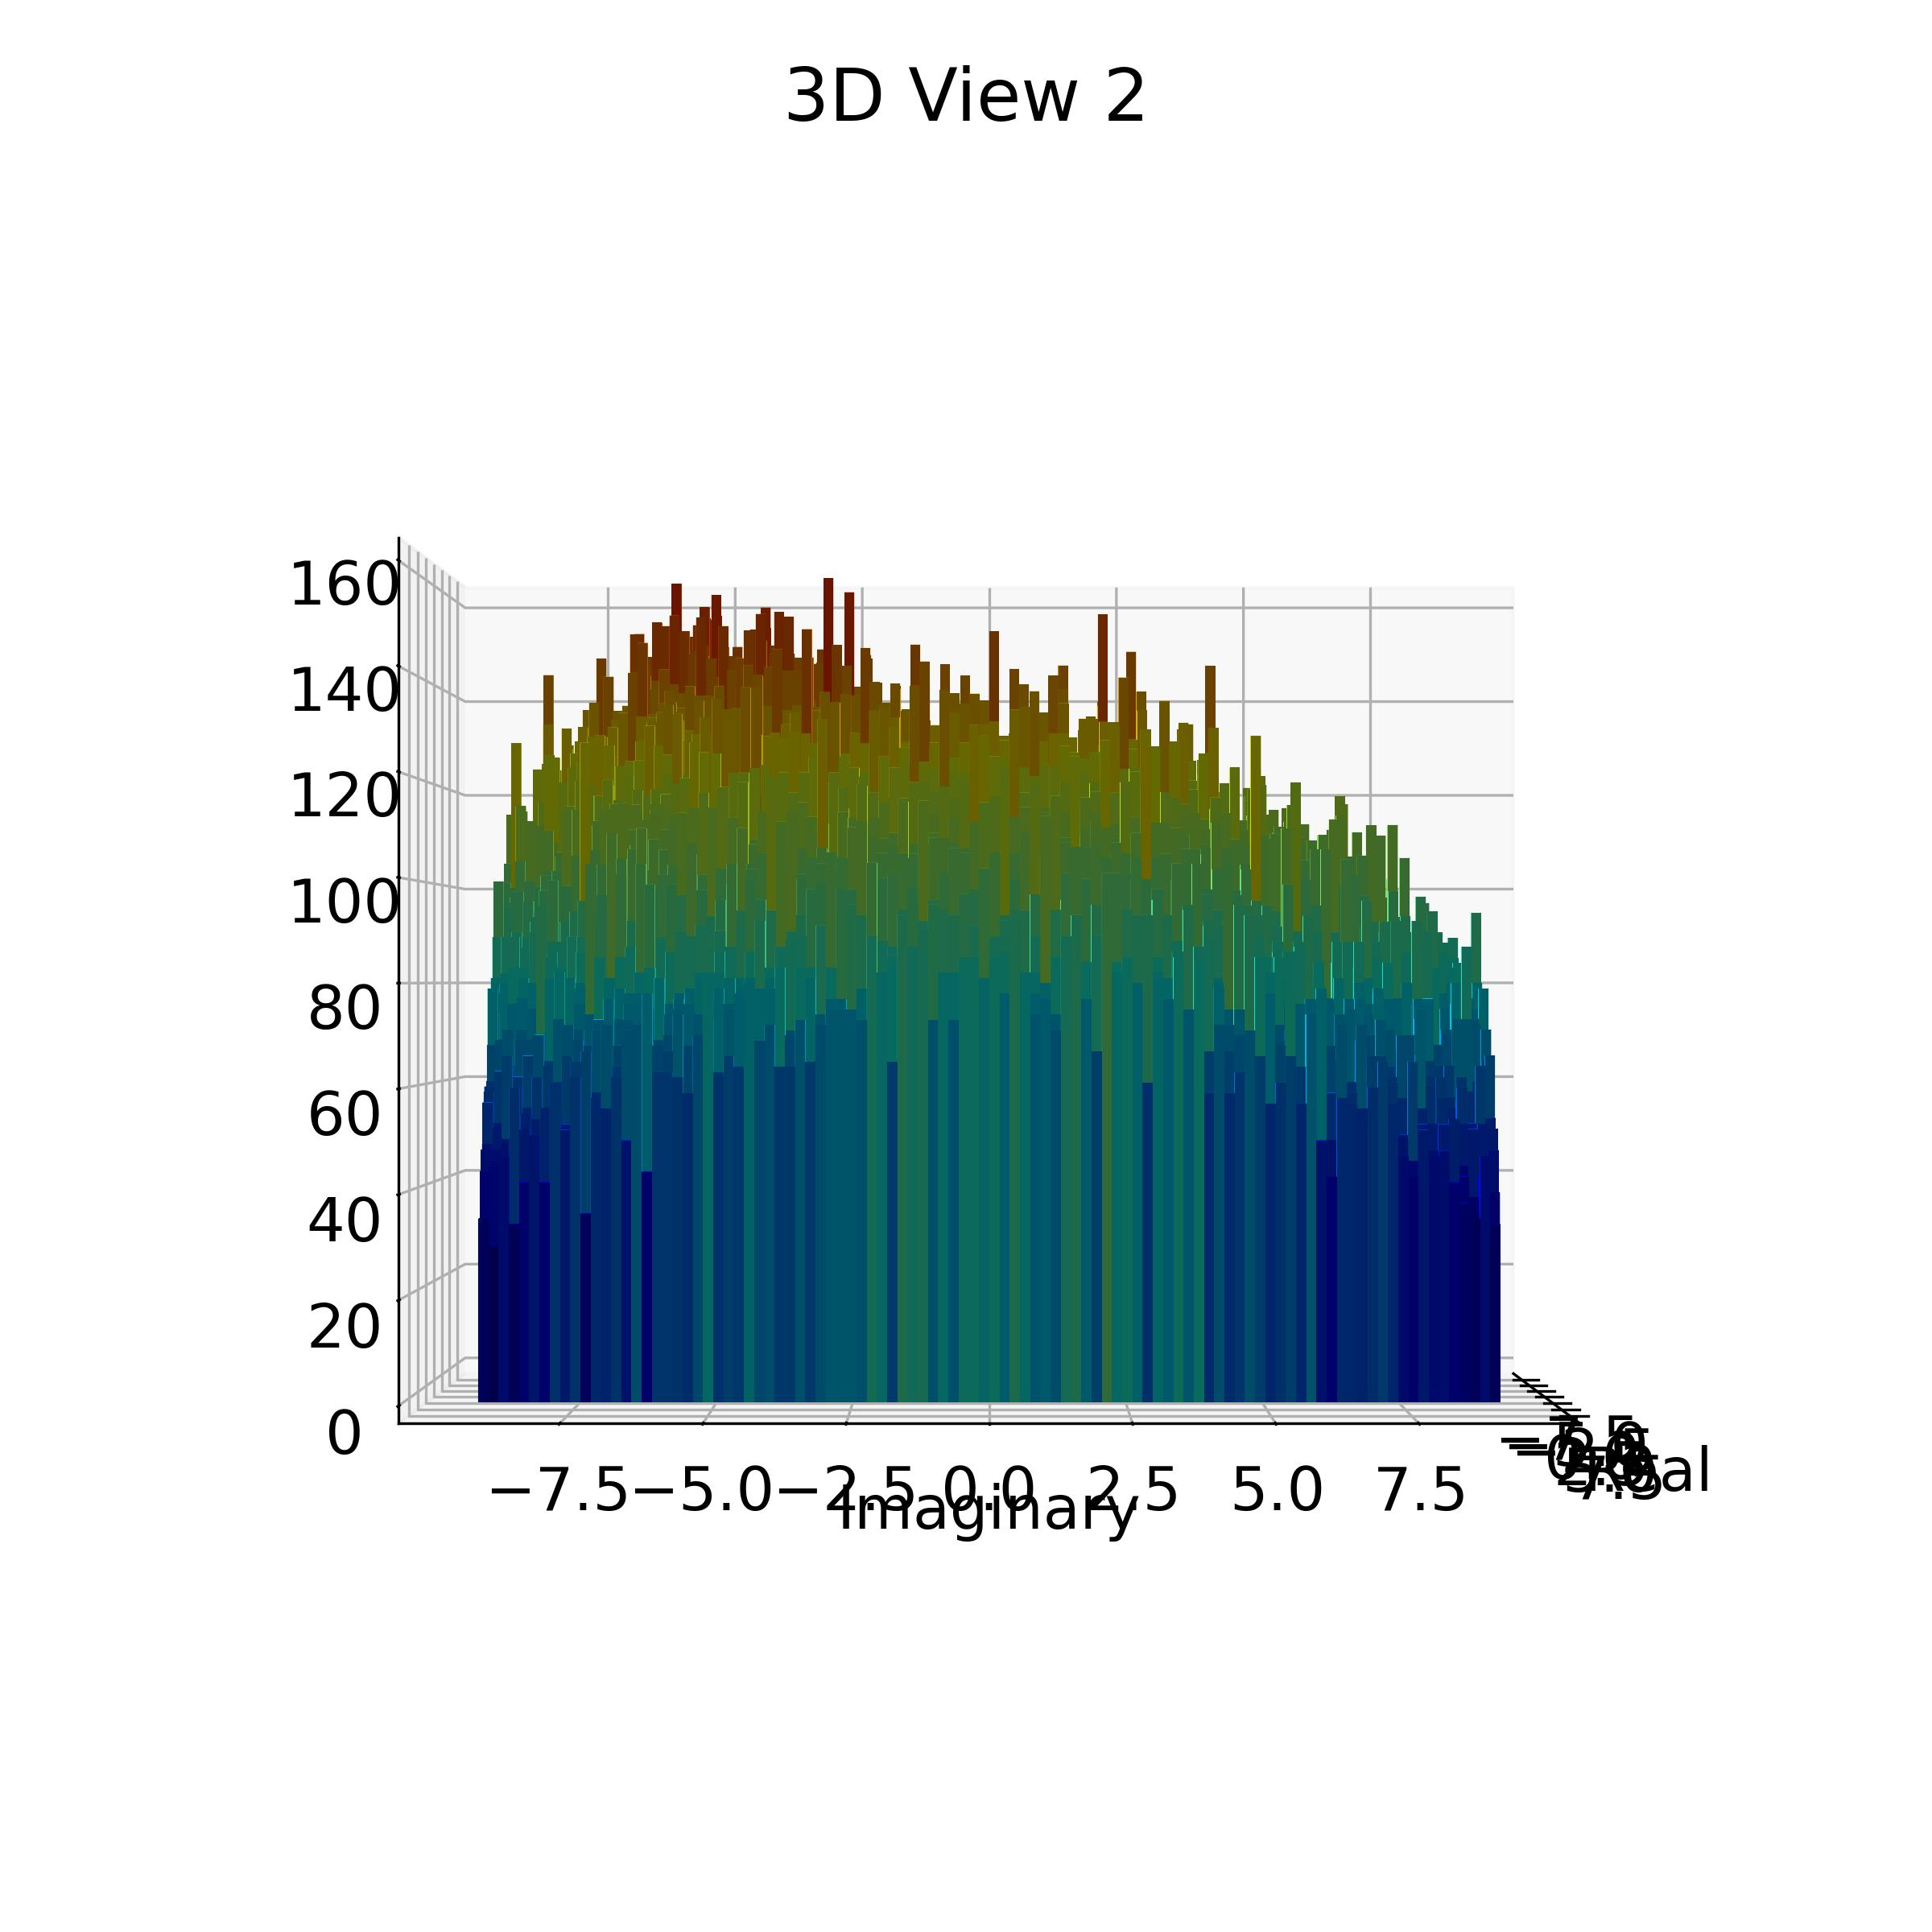
\includegraphics[width=1\linewidth]{images/demo/smf/smf_8.jpg} (i) \\
        }
        \end{minipage}
        \hfill
        \begin{minipage}[h]{0.49\linewidth}
        \center{
            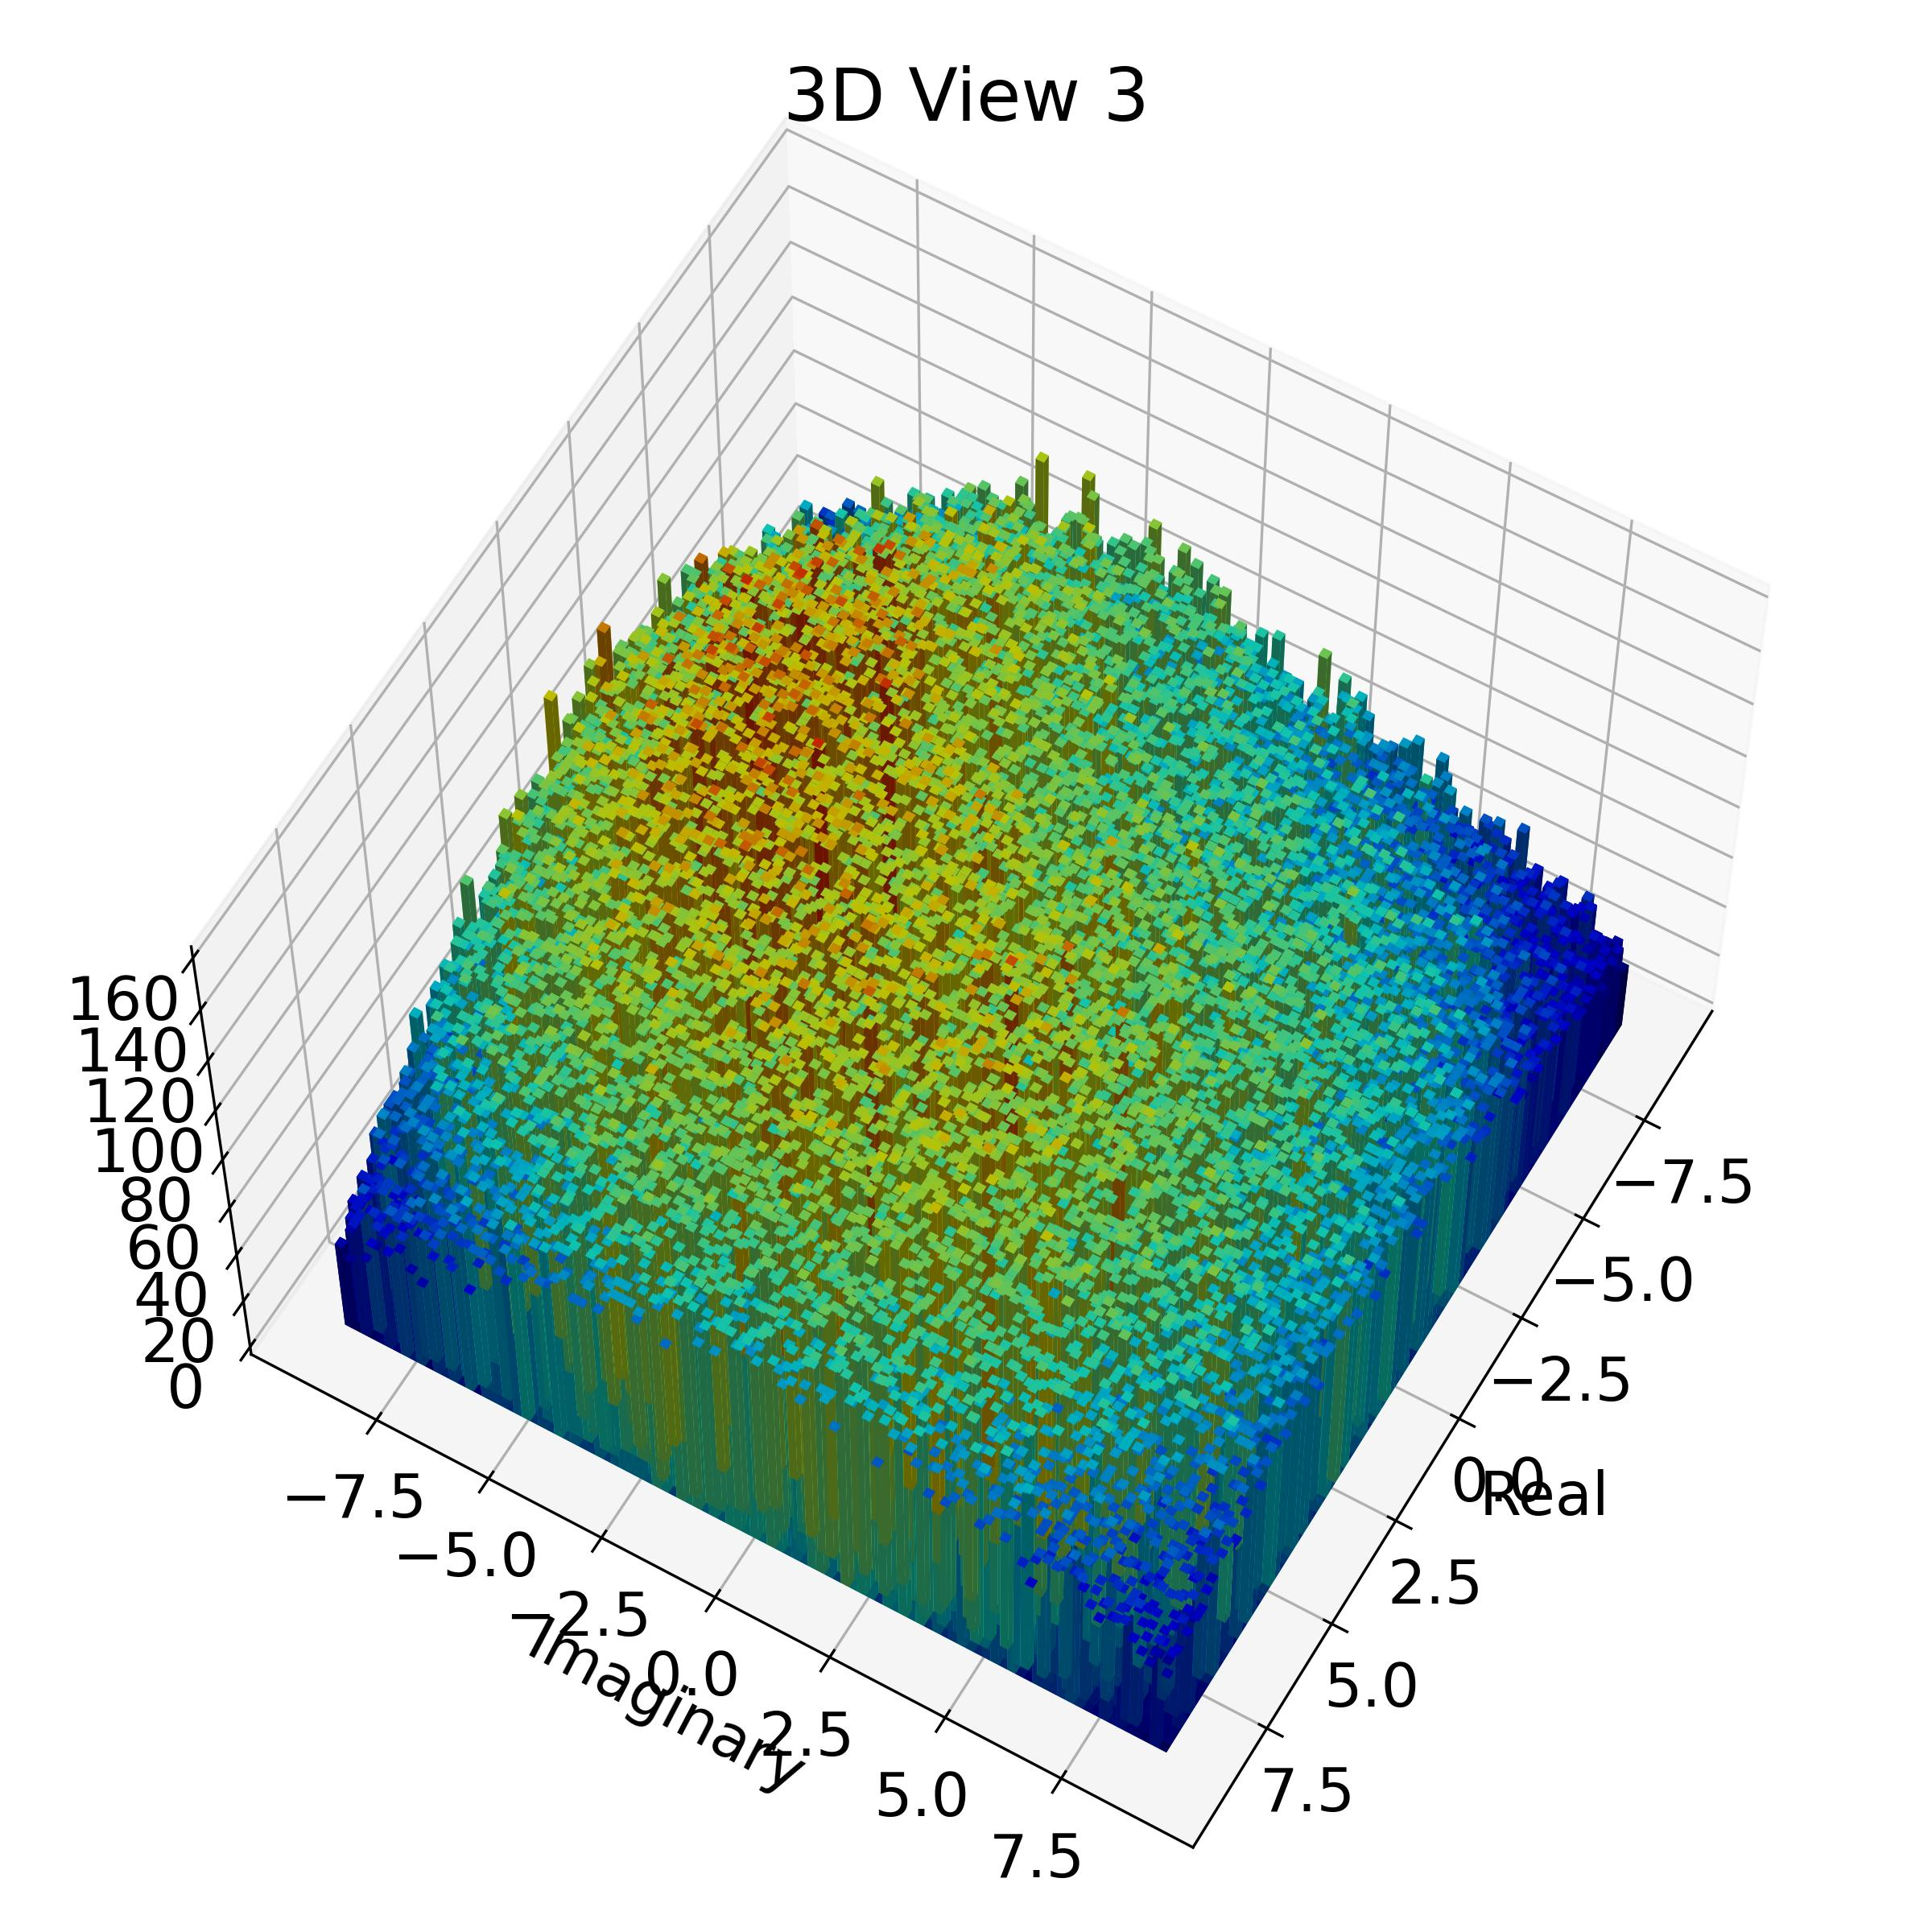
\includegraphics[width=1\linewidth]{images/demo/smf/smf_9.jpg} (j)
        }
        \end{minipage}
    \end{minipage}
    \caption{Signal propagation with parameters: $6 \times 80$ $[\textrm{km}]$ spans of \gls{smf}, attenuation coefficient of $\alpha = 0.2$ $[\textrm{dB}/\textrm{km}]$, EDFA noise figure 4.5 \textrm{[dB]}, a dispersion coefficient of $D = 16.8$ $\textrm{ps}/[\textrm{nm} \cdot \textrm{km}]$, and a nonlinear coefficient of $\gamma = 1.2$ $[\textrm{W} \cdot \textrm{km}]^{-1}$, average signal power $P_{ave} = 10$ $\textrm{dBm}$, 64-\gls{qam} format. \textbf{(a)} Original image. \textbf{(b)} Image post-propagation without equalisation. \textbf{(c)} Image after \gls{cdc} and \gls{npe}. \textbf{(d)} and \textbf{(e)} \gls{dbp} with 2 and 3 steps per span, respectively. \textbf{(f)} Image after \gls{nn} equalisation for received symbols. \textbf{(g)} to \textbf{(j)} Various constellation diagram representations.}
    \label{fig:demo_smf}
\end{figure}
\end{landscape}


Figure~\ref{fig:demo_twc} illustrates signal propagation through a system with the following parameters: spans of $10 \times 50$ $[\textrm{km}]$ using \gls{twc} fibre, an attenuation coefficient $\alpha = 0.2$ $[\textrm{dB}/\textrm{km}]$, an EDFA noise figure of 4.5 $[\textrm{dB}]$, a dispersion coefficient $D = 2.8$ $\textrm{ps}/[\textrm{nm} \cdot \textrm{km}]$, and a nonlinear coefficient $\gamma = 2.5$ $[\textrm{W} \cdot \textrm{km}]^{-1}$. The average signal power is set at $P_{ave} = 5$ $\textrm{dBm}$, and the modulation format is \gls{qpsk}. The figure showcases various stages of the signal, from the original image to different processing methods, including propagation without equalisation, \gls{cdc} and \gls{npe} application, \gls{dbp} with different steps per span, and equalisation using \gls{nn}. Additionally, it features different constellation diagram representations.


Figure~\ref{fig:demo_smf} presents signal propagation in a setup characterized by: spans of $6 \times 80$ $[\textrm{km}]$ using \gls{smf}, an attenuation coefficient $\alpha = 0.2$ $[\textrm{dB}/\textrm{km}]$, an EDFA noise figure of 4.5 $[\textrm{dB}]$, a dispersion coefficient $D = 16.8$ $\textrm{ps}/[\textrm{nm} \cdot \textrm{km}]$, and a nonlinear coefficient $\gamma = 1.2$ $[\textrm{W} \cdot \textrm{km}]^{-1}$. The average signal power stands at $P_{ave} = 10$ $\textrm{dBm}$, utilizing a 64-\gls{qam} format. The visualizations in the figure encompass the original image and its evolutions after several processing techniques, such as post-propagation without equalisation, the effects of \gls{cdc} and \gls{npe}, \gls{dbp} at varying steps per span, and \gls{nn} equalisation. The figure concludes with different views of the constellation diagram.




\section{Conclusion}

Through this live demonstration, participants can explore the capabilities and benefits of the HpCom library and better understand the impact of various parameters and techniques on signal quality in optical communication systems. By directly observing the results of their choices, participants will gain a better understanding of the complexities of optical signal transmission and the opportunities for improvement.
